%% LyX 2.1.4 created this file.  For more info, see http://www.lyx.org/.
%% Do not edit unless you really know what you are doing.
\documentclass[oneside,english,russian]{scrbook}
\usepackage[T2A,T1]{fontenc}
\usepackage[utf8]{inputenc}
\usepackage[a4paper]{geometry}
\geometry{verbose,tmargin=2cm,bmargin=2.5cm,lmargin=2cm,rmargin=2cm}
\setcounter{secnumdepth}{3}
\setcounter{tocdepth}{3}
\usepackage{color}
\usepackage{babel}
\usepackage{array}
\usepackage{verbatim}
\usepackage{latexsym}
\usepackage{float}
\usepackage{booktabs}
\usepackage{mathrsfs}
\usepackage{mathtools}
\usepackage{url}
\usepackage{amsmath}
\usepackage{amsthm}
\usepackage{amssymb}
\usepackage{graphicx}
\usepackage{esint}
\usepackage[unicode=true,pdfusetitle,
 bookmarks=true,bookmarksnumbered=false,bookmarksopen=true,bookmarksopenlevel=1,
 breaklinks=false,pdfborder={0 0 1},backref=false,colorlinks=true]
 {hyperref}
\usepackage{breakurl}
\usepackage{bm}

\makeatletter

%%%%%%%%%%%%%%%%%%%%%%%%%%%%%% LyX specific LaTeX commands.
\DeclareRobustCommand{\cyrtext}{%
  \fontencoding{T2A}\selectfont\def\encodingdefault{T2A}}
\DeclareRobustCommand{\textcyr}[1]{\leavevmode{\cyrtext #1}}
\AtBeginDocument{\DeclareFontEncoding{T2A}{}{}}

%% Special footnote code from the package 'stblftnt.sty'
%% Author: Robin Fairbairns -- Last revised Dec 13 1996
\let\SF@@footnote\footnote
\def\footnote{\ifx\protect\@typeset@protect
    \expandafter\SF@@footnote
  \else
    \expandafter\SF@gobble@opt
  \fi
}
\expandafter\def\csname SF@gobble@opt \endcsname{\@ifnextchar[%]
  \SF@gobble@twobracket
  \@gobble
}
\edef\SF@gobble@opt{\noexpand\protect
  \expandafter\noexpand\csname SF@gobble@opt \endcsname}
\def\SF@gobble@twobracket[#1]#2{}
%% Because html converters don't know tabularnewline
\providecommand{\tabularnewline}{\\}

%%%%%%%%%%%%%%%%%%%%%%%%%%%%%% Textclass specific LaTeX commands.
 \theoremstyle{definition}
 \newtheorem*{defn*}{\protect\definitionname}
  \theoremstyle{remark}
  \newtheorem*{rem*}{\protect\remarkname}
  \theoremstyle{plain}
  \newtheorem*{cor*}{\protect\corollaryname}
  \theoremstyle{definition}
  \newtheorem*{example*}{\protect\examplename}
  \theoremstyle{remark}
  \newtheorem*{claim*}{\protect\claimname}
  \theoremstyle{definition}
  \ifx\thechapter\undefined
    \newtheorem{example}{\protect\examplename}
  \else
    \newtheorem{example}{\protect\examplename}[chapter]
  \fi
  \theoremstyle{plain}
  \newtheorem*{prop*}{\protect\propositionname}
  \theoremstyle{definition}
  \newtheorem*{xca*}{\protect\exercisename}
  \theoremstyle{plain}
  \newtheorem*{thm*}{\protect\theoremname}
 \newenvironment{solution}
   {\renewcommand\qedsymbol{$\lrcorner$}
    \begin{proof}[\solutionname]}
   {\end{proof}}
  \theoremstyle{definition}
  \ifx\thechapter\undefined
    \newtheorem{xca}{\protect\exercisename}
  \else
    \newtheorem{xca}{\protect\exercisename}[chapter]
  \fi
\newenvironment{lyxcode}
{\par\begin{list}{}{
\setlength{\rightmargin}{\leftmargin}
\setlength{\listparindent}{0pt}% needed for AMS classes
\raggedright
\setlength{\itemsep}{0pt}
\setlength{\parsep}{0pt}
\normalfont\ttfamily}%
 \item[]}
{\end{list}}
  \theoremstyle{plain}
  \newtheorem*{assumption*}{\protect\assumptionname}
  \theoremstyle{remark}
  \newtheorem*{notation*}{\protect\notationname}

\@ifundefined{date}{}{\date{}}
%%%%%%%%%%%%%%%%%%%%%%%%%%%%%% User specified LaTeX commands.
%\usepackage{nicefrac}
%\usepackage{colortbl}
%\usepackage[noend]{algpseudocode}
%\usepackage{xypic}
\usepackage{eso-pic}

%\renewenvironment{example*}
%                  {\renewcommand\qedsymbol{$\lrcorner$}
%                   \begin{proof}[Пример]}
%                  {\end{proof}}

%\usepackage[columns=1,itemlayout=singlepar,totoc=true]{idxlayout}

\usepackage[columns=1,itemlayout=singlepar,totoc=true]{idxlayout}

\@addtoreset{chapter}{part}
\DeclareMathOperator{\Int}{Int}
\DeclareMathOperator{\rk}{rk}
\DeclareMathOperator{\tr}{tr}
\DeclareMathOperator{\cdf}{cdf}
\DeclareMathOperator{\ecdf}{ecdf}
\DeclareMathOperator{\qnt}{qnt}
\DeclareMathOperator{\pdf}{pdf}
\DeclareMathOperator{\pmf}{pmf}
\DeclareMathOperator{\dom}{dom}
\DeclareMathOperator{\bias}{bias}
\DeclareMathOperator{\MSE}{MSE}
\DeclareMathOperator{\med}{med}
\DeclareMathOperator{\Exp}{Exp}
\DeclareMathOperator{\Bin}{Bin}
\DeclareMathOperator{\Ber}{Ber}
\DeclareMathOperator{\Geom}{Geom}
\DeclareMathOperator{\Pois}{Pois}
\DeclareMathOperator*{\argmax}{argmax}
\DeclareMathOperator{\im}{im}
\DeclareMathOperator{\cov}{cov}
\DeclareMathOperator{\cor}{cor}
\DeclareMathOperator{\sign}{sign}
\DeclareMathOperator{\Lin}{Lin}
\DeclareMathOperator{\SE}{SE}
\DeclareMathOperator{\SD}{SD}
\DeclareMathOperator*{\argmin}{argmin}
\DeclareMathOperator*{\proj}{proj}
\DeclareMathOperator{\colspace}{colspace}
\DeclareMathOperator*{\plim}{plim}
\DeclareMathOperator{\corr}{corr}
\DeclareMathOperator{\supp}{supp}

\newcommand{\bigperp}{%
  \mathop{\mathpalette\bigp@rp\relax}%
  \displaylimits
}

\newcommand{\bigp@rp}[2]{%
  \vcenter{
    \m@th\hbox{\scalebox{\ifx#1\displaystyle2.1\else1.5\fi}{$#1\perp$}}
  }%
}

\newcommand{\bignparallel}{%
  \mathop{\mathpalette\bignp@rp\relax}%
  \displaylimits
}

\newcommand{\bignp@rp}[2]{%
  \vcenter{
    \m@th\hbox{\scalebox{\ifx#1\displaystyle2.1\else1.5\fi}{$#1\nparallel$}}
  }%
}

\renewenvironment{cases}{%
 \begin{dcases}%
}{%
 \end{dcases}%\kern-\nulldelimiterspace%
}

\newcommand{\notimplies}{%
  \mathrel{{\ooalign{\hidewidth$\not\phantom{=}$\hidewidth\cr$\implies$}}}}

\newcommand{\notiff}{%
  \mathrel{{\ooalign{\hidewidth$\not\phantom{"}$\hidewidth\cr$\iff$}}}}

\AtBeginDocument{
  \def\labelitemii{\(\Diamond\)}
  \def\labelitemiii{\(\Box\)}
}

\makeatother

  \addto\captionsenglish{\renewcommand{\assumptionname}{Assumption}}
  \addto\captionsenglish{\renewcommand{\claimname}{Claim}}
  \addto\captionsenglish{\renewcommand{\corollaryname}{Corollary}}
  \addto\captionsenglish{\renewcommand{\definitionname}{Definition}}
  \addto\captionsenglish{\renewcommand{\examplename}{Example}}
  \addto\captionsenglish{\renewcommand{\exercisename}{Exercise}}
  \addto\captionsenglish{\renewcommand{\notationname}{Notation}}
  \addto\captionsenglish{\renewcommand{\propositionname}{Proposition}}
  \addto\captionsenglish{\renewcommand{\remarkname}{Remark}}
  \addto\captionsenglish{\renewcommand{\theoremname}{Theorem}}
  \addto\captionsrussian{\renewcommand{\assumptionname}{Предположение}}
  \addto\captionsrussian{\renewcommand{\claimname}{Утверждение}}
  \addto\captionsrussian{\renewcommand{\corollaryname}{Следствие}}
  \addto\captionsrussian{\renewcommand{\definitionname}{Определение}}
  \addto\captionsrussian{\renewcommand{\examplename}{Пример}}
  \addto\captionsrussian{\renewcommand{\exercisename}{Упражнение}}
  \addto\captionsrussian{\renewcommand{\notationname}{Обозначение}}
  \addto\captionsrussian{\renewcommand{\propositionname}{Предложение}}
  \addto\captionsrussian{\renewcommand{\remarkname}{Замечание}}
  \addto\captionsrussian{\renewcommand{\theoremname}{Теорема}}
  \providecommand{\assumptionname}{Предположение}
  \providecommand{\claimname}{Утверждение}
  \providecommand{\corollaryname}{Следствие}
  \providecommand{\definitionname}{Определение}
  \providecommand{\examplename}{Пример}
  \providecommand{\exercisename}{Упражнение}
  \providecommand{\notationname}{Обозначение}
  \providecommand{\propositionname}{Предложение}
  \providecommand{\remarkname}{Замечание}
  \providecommand{\theoremname}{Теорема}
 \addto\captionsenglish{\renewcommand{\solutionname}{Solution}}
 \addto\captionsrussian{\renewcommand{\solutionname}{Решение}}
 \providecommand{\solutionname}{Решение}

\begin{document}
\global\long\def\N{\mathrm{N}}
\global\long\def\P{\mathsf{P}}
\global\long\def\E{\mathsf{E}}
\global\long\def\D{\mathsf{D}}
\global\long\def\O{\Omega}
\global\long\def\F{\mathcal{F}}
\global\long\def\K{\mathsf{K}}
%\global\long\def\Ascr{\mathscr{A}}
\global\long\def\Ascr{A}
\global\long\def\Pcal{\mathcal{P}}
\global\long\def\th{\theta}
\global\long\def\toas{\xrightarrow{\textrm{a.s.}}}
\global\long\def\toP{\xrightarrow{\P}}
\global\long\def\tod{\xrightarrow{\mathrm{d}}}
\global\long\def\iid{\mathrm{i.i.d.}}
\global\long\def\T{\mathsf{T}}
\global\long\def\L{\mathsf{L}}
\global\long\def\dd#1#2{\frac{\mathrm{d}#1}{\mathrm{d}#2}}
\global\long\def\a{\alpha}
\global\long\def\b{\beta}
\global\long\def\t{\mathrm{t}}
\global\long\def\RR{\mathbb{R}}
\global\long\def\d{\,\mathrm{d}}
\global\long\def\U{\mathrm{U}}
\global\long\def\thb{\boldsymbol{\theta}}
\global\long\def\I{\mathrm{I}}
\global\long\def\II{\mathrm{II}}
\global\long\def\ein{\mathbf{1}}
\global\long\def\pv{p\text{-value}}
\global\long\def\MLE{\mathrm{MLE}}
\global\long\def\indep{\perp\!\!\!\perp}
\global\long\def\xib{\boldsymbol{\xi}}
\global\long\def\Pscr{\mathscr{P}}
\global\long\def\m{\mathsf{m}}
\global\long\def\FWER{\mathrm{FWER}}
\global\long\def\weak{\mathrm{weak}}
\global\long\def\H{\mathbf{H}}
\global\long\def\strong{\mathrm{strong}}
\global\long\def\X{\mathbf{X}}
\global\long\def\bb{\mathbf{b}}
\global\long\def\y{\mathbf{y}}
\global\long\def\eb{\boldsymbol{\epsilon}}
\global\long\def\Db{\boldsymbol{\Delta}}
\global\long\def\M{\mathbf{M}}
\global\long\def\eb{\boldsymbol{\epsilon}}
\global\long\def\S{\mathbf{S}}
\global\long\def\R{\mathbf{R}}
\global\long\def\A{\mathbf{A}}
\global\long\def\B{\mathbf{B}}
\global\long\def\OLS{\mathrm{OLS}}
\global\long\def\mb{\boldsymbol{\mu}}
\global\long\def\Sb{\boldsymbol{\Sigma}}
\global\long\def\Ib{\mathbf{I}}
\global\long\def\SST{\mathrm{SST}}
\global\long\def\SSR{\mathrm{SSR}}
\global\long\def\SSE{\mathrm{SSE}}
\global\long\def\x{\mathbf{x}}
\global\long\def\V{\mathbf{V}}
\global\long\def\etab{\boldsymbol{\eta}}
\global\long\def\Ell{\mathscr{L}}
\global\long\def\p{\mathbf{p}}
\global\long\def\Pb{\mathbf{P}}
\global\long\def\z{\mathbf{z}}
\global\long\def\C{\mathbf{C}}
\global\long\def\W{\mathbf{W}}





\chapter{Проверка гипотез}
%Тут должно быть про определение критерия и построение его через статистику критерия.

\section{Общие сведения}

\subsection{Примеры гипотез}
Пусть $H_0$ --- это гипотеза (\textbf{h}ypothesis), т.е. некоторое предположение о случайной величине $\xi$, которое мы хотим проверить (модель --- это предположение, которое считается верным без проверки).
Она называется нулевой (null hypothesis), потому что позднее появится альтернативная к ней.

Важно, что гипотеза --- предположение о неизвестном законе распределения $\xi$, а не о выборке.

Например, гипотеза о том мат.ож. давления до и после приема лекарств одинаково. Или гипотеза о том, что распределение ошибки прибора нормальное, или о том, что распределение генератора псевдослучайных чисел равномерное на [0,1], или что . Или о том, что зависимости между временем на смотрением анимэ и успехами в учебе нет. Тут прослеживается такая особенность: в гипотезе обычно предполагается, что эффекта нет, так как решение принимается, если гипотеза отвергается.

\textbf{Задание}: Напишите, какую гипотезу вам было бы интересно проверить и какие данные для этого нужно было бы собрать?

\subsection{Критерий}
Для проверки гипотезы применяется критерий. Критерий --- это правило, по которому гипотеза либо отвергается, либо не отвергается. Про построение такого правила --- позже.

Правило строится на основе выборки. Разумное решение:
нам нужно построить правило, которое, как уже говорилось, показывает, насколько выборка отличается от тех предположений, которые постулируются в гипотезе. Если отличается сильно, то гипотезы отвергается.

Измерять отличие удобно в числах.
Поэтому вводится статистика критерия (функция от выборки, на основе которой строится критерий) $t=t(x_1,\ldots,x_n)$, которая выборке сопоставляет число.

Например, гипотеза про то, что $H_{0}:\E\xi=0$ (например, условия тренировки не влияют на результат (средняя разница в результатах нулевая)).
В этом случае, 0 --- ожидаемое значение (expected), выборочное среднее $\bar{x}$ --- наблюдаемое значение (observed). Их разница как раз измеряет отличие. Однако, просто по разнице не сказать, отличие большое или нет.
И вообще, числа могут получиться случайно, на их основе теорию не построить.

На основе результатов критерия принимают решения. Например, если лекарство показало эффективность (гипотезу о том, что оно неэффективно, отвергли), то оно запускают в производство.

\subsection{Нет безошибочных решений}

Проблема: случайно может произойти что угодно, т.е. безошибочных решений практически не бывает. Приходится задавать максимальный уровень вероятности ошибки, на который можно согласиться при принятии решения.

Задаем маленький уровень значимости (significance level) $0<\alpha<1$ и соглашаемся, что с вероятностью $\alpha$ будем принимать неправильное решение.

Что такое маленький? Это зависит от критичности ошибки при принятии решения. Например, ...

\textbf{Задание}: Придумайте ситуацию (гипотезу), когда на вероятность ошибочного решение больше 0.001 вы бы точно не согласились.
Вторая ситуация --- когда согласились бы и на 0.2, но, пожалуй, не больше.

\subsection{Статистический критерий}
Чтобы построить теорию и отвечать на вопрос, маленькое или большое значение статистики критерия, отвергать гипотезу или нет, нужно перейти на теоретический язык.
Т.е., нужно рассматривать абстрактную выборку, 'до эксперимента', где $x_i$ --- одинаково распределенные независимые случайные величины с тем же распределением, что и у $\xi$.

Таким образом, и статистика критерия $t=t(x_1,\ldots,x_n)$ --- тоже случайная величина.
Если верна $H_0$, то $t$ имеет некоторое распределение и принимает некоторый диапазон значений.

Например, для модели $\xi\sim N(a,\sigma^2)$ и гипотезы $H_{0}:\E\xi=0$, статистика критерия $t = \sqrt{n}\bar{x}/\sigma$ имеет распределение $N(0,1)$. Видим, что возможны любые значения. Однако, если мы допускаем некоторую вероятность ошибочно отвергнуть верную нулевую гипотезу, то критерий можем построить.
Обычно главное --- контролировать эту вероятность.

Разбиваем значения статистики критерия на две части, доверительную и критическую область так, что
вероятность для статистика критерия попасть в критическую область равна $\alpha$.

\textbf{Задание}. Нарисуйте плотность распределения статистики критерия $t=\sqrt{n}\bar{x}/\sigma$ при условии, что верна нулевая гипотезы, и разбейте область значений на две части, доверительную и критическую. Сделайте это разумным образом, чтобы было разумно значения из критической области считать не соответствующими справедливости нулевой гипотезы.

\paragraph{Формальное определение}
Назовем критерием разбиение области значений статистики критерия на две части, ${\Ascr}^{(\text{крит})}_\alpha$ и ${\Ascr}^{(\text{дов})}_\alpha$, такие что вероятность ошибки первого рода
$\alpha_I=\P_{H_0} (t\in {\Ascr}^{(\text{крит})}_\alpha) = \alpha$.

После того как критерий построен, пользуемся им уже в режиме 'после эксперимента', когда выборка и значение статистики критерия --- числа. Если число $t$ попадает в критическую область, то гипотеза отвергается. Иначе --- не отвергается (но нельзя говорить, что принимается, это обсудим позднее).

Итак, важно (!): разбиение на доверительную и критическую область строится на теор. языке, для абстрактной выборки. А используется это разбиение уже для конкретной выборки, чисел.

Допустимо строить разбиение так, чтобы выполнялось $\alpha_I \leq \alpha$ (тогда критерий называется консервативным).

Часто удается построить только асимптотический критерий, когда $\alpha_I \rightarrow \alpha$ при $n\rightarrow \infty$. В этом случае критерий можно применять при достаточно (для критерия) большом объеме выборки, где допустимый объем выборки зависит от скорости сходимости.

Ниже более подробно.

\section{Схема построение критерия на основе статистики критерия}
%\paragraph{Схема построения критерия с помощью статистики критерия}
\begin{enumerate}
\item
Строим статистику критерия $t$ так, что:
\begin{itemize}
\item Cтатистика критерия $t$ должна измерять то, насколько выборка соответствует гипотезе.
В этом случае мы получаем значение статистики критерия для <<идеального соответствия>>.

Например, если гипотеза про математическое ожидание, то $t=\bar{x}-\E\xi$ подходит под это требование.
Если гипотеза про дисперсию, то соответствие правильнее измерять отношением и поэтому подошло бы $t=s^2/\D\xi$.

\begin{example*}
Пусть $H_{0}:\E\xi=a_{0}$; тогда $t=\bar{\mathbf{x}}-a_{0}$ и <<идеальное
значение>> $t=0$.
\end{example*}
\item Распределение $t$ при верной $H_{0}$ должно быть известно хотя бы
асимптотически. Из-за этого часто преобразовывают вариант меры несоответствия, приведенный выше.
Для $H_0:\, \E\xi = a_0$ в модели $\xi\sim N(a, \sigma^2)$ с известной дисперсией $\sigma^2$ удобно использовать статистику критерия $t=\sqrt{n}(\bar{\mathbf{x}}-a_{0})/\sigma \sim N(0,1)$.
\end{itemize}

\item
Строим разбиение области значений статистики критерия $t$ так, что: %
\begin{itemize}
\item $\P(t\in \Ascr_\alpha^{\text{крит}} )= \alpha$.

\item Если альтернативная гипотеза $H_{1}$ (см. про нее в след.разделе) не конкретизирована, то $\Ascr_\a^{\text{(крит)}}$ следует выбрать
так, чтобы она располагалась как можно дальше от идеального значения.

\begin{example*}
В случае $t\sim\N(0,1)$ при идеальном значении $0$, разумно определить $\Ascr_\a^{\text{(крит)}}$
<<на хвостах>> графика $\pdf_{\N(0,1)}$ симметрично по обе стороны
от 0 так, что для $\Ascr_\a^{\text{(крит)}}=(-\infty,-t_{\a})\cup(t_{\a},\infty)$
\[
\a/2=\int_{-\infty}^{-t_{\a}}\pdf_{\N(0,1)}(y)\d y=\int_{t_{\a}}^{+\infty}\pdf_{\N(0,1)}(y)\d y.
\]
 Иными словами,
\[
\a/2=1-\cdf_{\N(0,1)}(t_{1})\implies t_{1}=\cdf_{\N(0,1)}^{-1}(1-\a/2)
\]
и аналогично для $t_{0}$. Границы доверительной области часто называют критическими значениями.
\end{example*}
\item На будущее: если $H_{1}$ известна, то $\Ascr_\a^{\text{(крит)}}$ выбирается так,
чтобы максимизировать мощность критерия против альтернативы $H_{1}$, определения см. ниже.
\end{itemize}
\end{enumerate}

\subsection{Пример с числами}

Общая схема всех примеров будет как написано ниже.

Модель: (необязательно)

Гипотеза: $H_0: ...$

Статистика критерия $t = ...$:

Ее распределение при условии, что верная $H_0$: ... --- выписано распределение.

Дана выборка, дан уровень значимости.

Задание: проверить гипотезу, сказать, отвергается она или нет.

Как решать:

1) теор.часть, выборка абстрактная, уровень значимости $\alpha$ тоже произвольный. По виду статистики критерия вы понимаете, какое значение соответствует 'идеальному' соответствию данных гипотезе. Рисуете график плотности статистики критерия и разбиваете значения на доверит. и крит. части, чтобы вероятность попасть в крит. область была равна $\alpha$. В крит.область включаете значения, наиболее далекие от 'идеального'.

2) практическая часть, выборка состоит из чисел, уровень значимости --- конкретное число.
Подставляете в формулу статистики критерия числа, получаете число, обозначим $t_0$.
Затем считаем, чему равны критические значения (граница(ы) между критической и доверительной областями). Эти числа выражаются через обратную функцию распределения (это квантили). Значения можно вычислить  в R или Python, см. ниже приложение. Рисуем снова график плотности статистики критерия, отмечаем там найденные числа, показываем, где критическая). область, где доверительная. На основе того, куда попало $t_0$, делаем вывод, отвергается или нет нулевая гипотеза.

Ниже я буду давать три варианта, в зависимости от остатка деления дня рождения на 3. pdf всего, что рассказывалось, сейчас выложу в vk.

\textbf{Задание 1}: Провести эту схему (записать то, что выше, с самого начала, со слова Модель) для уже разобранного выше критерия со статистикой критерия $t=\sqrt{n}(\bar{\mathbf{x}}-a_{0})/\sigma$. Там дисперсия $\sigma^2$ предполагается известной. Пусть она равна 1.44. Гипотеза: $H_0: \E\xi = a_0$, где (0) $a_0 =-1$, (1) $0.5$, (2) $1$. Примените критерий для выборки (0,2,1,-1,-2) и уровня значимости (0) $\alpha = 0.05$, (1) $0.1$, (2)  $0.2$.

\textbf{Задание 2}: Провести эту схему для следующей постановки задачи.

Модель: $\xi$ имеет распределение Бернулли с неизвестным параметром, вероятностью успеха $p$. Напомню, что это означает, что она принимает значения 0 и 1, 1 (успех) с вероятностью $p$.

Гипотеза: $H_0: p=p_0$

Статистика критерия: \[
t=\sqrt{n}\frac{\hat{p}-p_{0}}{\sqrt{p_{0}(1-p_{0})}},
\]
где $\hat{p} = \bar{x}$, что логично, так как сумма значений выборки --- это в точности число успехов.

Ее распределение при условии, что $H_0$ верна: $t\tod\N(0,1)$ (т.е. это асимптотический критерий).

Дана выборка в виде: число успешных собеседований 45, неуспешных --- 55. Проверить гипотезу (0) $H_0: p = 0.45$, (1) $0.5$, (2) $0.4$, уровень значимости (0) $\alpha = 0.2$, (1) $0.05$, (2)  $0.1$.

Задание: проверить гипотезу, сказать, отвергается она или нет.


\textbf{Задание 3}: Провести эту схему для следующей постановки задачи.

Модель: нет (но предполагается, что $\xi$ принимает конечное число значений).

Гипотеза:
\[
H_{0}:\Pcal_\xi=\Pcal_{0},\text{ где }\Pcal_{0}:\begin{pmatrix}x_{1}^{*} & \dots & x_{k}^{*}\\
p_{1} & \dots & p_{k}
\end{pmatrix}.
\]

Статистика критерия: \[
T=\sum_{i=1}^{k}\frac{(n_{i}-np_{i})^{2}}{np_{i}}.
\]
Здесь такие обозначения: выборка $\mathbf{x}$ сгруппирована, т.е. каждому $x_{i}^{*}$ сопоставляем \emph{наблюдаемую}
абсолютную частоту $n_{i}$; $np_{i}$ --- \emph{ожидаемая}
абсолютная частота.

Ее распределение при условии, что $H_0$ верна: $T\tod\chi^{2}(k-1)$.
 (т.е. это асимптотический критерий). По поводу свойств и вида плотности распределения хи-квадрат отсылаем к википедии \url{https://ru.wikipedia.org/wiki/%D0%A0%D0%B0%D1%81%D0%BF%D1%80%D0%B5%D0%B4%D0%B5%D0%BB%D0%B5%D0%BD%D0%B8%D0%B5_%D1%85%D0%B8-%D0%BA%D0%B2%D0%B0%D0%B4%D1%80%D0%B0%D1%82}.

Дана выборка в виде: число успешных собеседований 45, неуспешных --- 55. Проверить гипотезу, что это распределение Бернулли с $p=0.05$. Проверить для значений $\alpha$ от 0.01 до 0.99 с шагом 0.01.

Задание: проверить гипотезу, сказать, отвергается она или нет. Когда надоест перебирать уровни значимости, найдите такое пороговое значение, называемое $p$-значение, что при меньших уровнях значимости гипотеза не отвергается, а при бОльших --- отвергается.
%\section{Ошибки первого и второго рода}
%\begin{defn*}[Ошибки I-го и II-го родов]
%Пусть мы проверяем нулевую гипотезу $H_{0}$. Зафиксируем альтернативную гипотезу $H_{1}$ --- такое отклонение
%от $H_{0}$, что его обнаружение важно для нас. Тогда
%\begin{itemize}
%\item ошибка \emph{I-го рода} есть отвержение $H_{0}$, при верной $H_{0}$; соответствующая
%вероятность есть
%\[
%\a_{\mathrm{I}}:=\P_{H_{0}}(\mathbf{x}\in\Ascr_{\text{крит}}^{(\a)}).
%\]
%
%
%\begin{rem*}
%Для точного критерия вероятность $\a_{\mathrm{I}}$ совпадает с уровнем
%значимости $\a$.
%\end{rem*}
%\item ошибка \emph{II-го рода} есть не отвержение $H_{0}$ при верной $H_{1}$;
%соответствующая вероятность есть
%\[
%\a_{\mathrm{II}}:=\P_{H_{1}}(\mathbf{x}\in\Ascr_{\text{дов}}^{(\a)}).
%\]
%
%\end{itemize}
%\end{defn*}
%
%\begin{defn*}
%\emph{Мощность} критерия против альтернативы есть
%\[
%\b:=1-\a_{\mathrm{II}}=1-\P_{H_{1}}(\mathbf{x}\in\Ascr_{\text{дов}}^{(\a)})=\P_{H_{1}}(\mathbf{x}\in\Ascr_{\text{крит}}^{(\a)}).
%\]
%
%
%Иными словами, это способность критерия отличать $H_{1}$ от $H_{0}$.
%\end{defn*}
%
%\begin{defn*}
%Критерий называется \emph{состоятельным}, если $\b\to1$.\end{defn*}
%\begin{rem*}
%Утверждать об \emph{отвержении} гипотезы можно с вероятностью ошибки
%$\a$ (достаточно малой); утверждать о \emph{принятии} гипотезы можно
%с вероятностью ошибки $\a_{\mathrm{II}}$ --- не контролируемой и
%могущей быть довольно большой. Поэтому гипотезу $H_0$ можно только
%отвергать или не отвергать, так как мы контролируем ошибку неправильного решения (отвергнуть).
%Принимать гипотезу нельзя, так как мы не контролируем, вообще говоря, ошибку неправильного решения в случае принятия гипотезы.
%\end{rem*}
%
%\begin{rem*}
%В связи с введенным понятием мощности можно описать две проблемы:
%\begin{itemize}
%\item
%проблема маленьких объемов выборки состоит в том, что в этом случае мощность маленькая и критерий не заметит отличие от $H_1$ от $H_0$, т.е. с большой вероятностью не отвергнет $H_0$, хотя будет верна $H_1$;
%\item
%как ни странно, но есть также проблема слишком больших объемов выборки, когда мощность слишком большая, т.е. критерий может отвергнуть $H_0$ с большой вероятностью, даже если она <<почти>> верна (например, из-за ошибок округления).
%\end{itemize}
%\end{rem*}
%
%Заметим, что вероятность ошибки первого рода $\alpha_I$ фиксирована (как минимум, она ограничена сверху выбранным значением $\alpha$, в то время как $\a_{\mathrm{II}} = \a_{\mathrm{II}}(\alpha, n, H_1)$. Ниже продемонстрируем эту зависимость на примере.
%
%\begin{example*}
%\label{exa:h0-h1}Пусть $\xi\sim\N(a,\sigma^{2})$, $\sigma^{2}$
%известна --- это модель. Гипотезы имеют вид $H_{0}:a=a_{0},\ H_{1}:a=a_{1}$. Тогда
%\[
%t=\dfrac{\sqrt{n}\left(\bar{\mathbf{x}}-a_{0}\right)}{\sigma}\sim\N(0,1)\text{ при верной }H_{0}.
%\]
% В то же время, поскольку при верной $H_{1}$, $\E\bar{\mathbf{x}}=1/n\cdot\sum_{i=1}^{n}\xi_{i}=n/n\cdot a_{1}$
%то
%\[
%\E t=\frac{\sqrt{n}\left(a_{1}-a_{0}\right)}{\sigma}\implies t\sim\N\left(\frac{\sqrt{n}\left(a_{1}-a_{0}\right)}{\sigma},1\right)\text{ при верной }H_{1}.
%\]
%(дисперсия, конечно, не меняется при сдвиге).
%
%\begin{figure}[H]
%\centering{}\includegraphics[width=0.5\textwidth]{fig/h0_h1}\caption{Плотности распределения $t$ (неоптимальное разбиение)}
%\end{figure}
%
%
%Чтобы минимизировать $\a_{\mathrm{II}}$, логично определить $\Ascr_{\text{крит}}$
%только на одном хвосте --- с той стороны, где находится альтернатива.
%
%\begin{figure}[H]
%\centering{}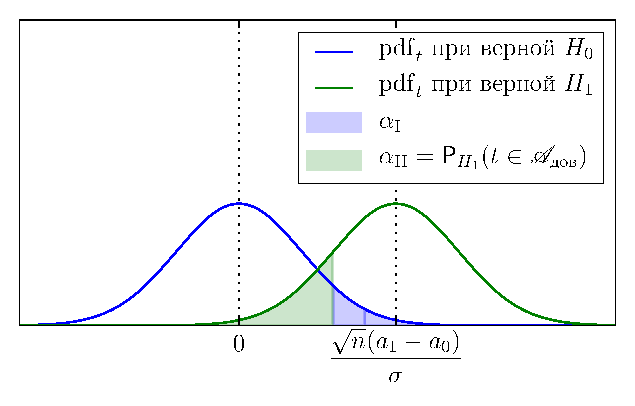
\includegraphics[width=0.5\textwidth]{fig/h0_h1-opt}\caption{Плотности распределения $t$ (оптимальное разбиение)}
%\end{figure}
%
%Таким образом, мы увидели, что если известна альтернатива, то можно выбирать критерий
%(= разбиение на доверительную и критическую области; статистика критерия — лишь удобной
%средство для этого), более мощный против именно этой альтернативы. И вообще, разные критерии для одной и той же основной гипотезы сравниваются по мощности против интересующей нас
%альтернативы.
%
%Помимо этого, по рисунку видно, что ошибка второго рода $\a_{\mathrm{II}}$ уменьшается при (1) увеличении
%ошибки первого рода (уровня значимости $\a$) (поэтому мы ее выбираем максимальной из всех
%допустимых); (2) увеличении объема выборки (если $\a_{\mathrm{II}}$ стремится к нулю при увеличении объема
%выборки, то критерий называется состоятельным после данной альтернативы) и (3) увеличении
%разницы между $H_0$ и $H_1$ в том же смысле, в каком статистика критерия измеряет разницу между выборкой и нулевой гипотезой. Напомним, что мощность критерия против некоторой альтернативы (чего-то
%отличного от основной гипотезы) говорит нам о том, насколько хорошо критерий обнаруживает
%это отличие.
%
%\end{example*}
%%\begin{rem*}
%%Помимо этого, по рисунку видно, что минимизировать $\a_{\mathrm{II}}$
%%(согласившись на б\'oльшую ошибку первого рода) можно сдвинув вправо
%%центр второй плотности, увеличив $n$.
%%
%%Аналогично, чем $a_{1}$ дальше от $a_{0}$, тем $\a_{\mathrm{II}}$
%%меньше. Стоит отметить, что $H_{1}$ не выбирается, но берется из
%%смысла задачи.
%%\end{rem*}
%%
%%\begin{example*}[С гранатами]
%%\begin{comment}
%%@xio: FIXME
%%\end{comment}
%%\end{example*}

\section{Понятие вероятностного уровня $p$-value.}
\begin{defn*}
\emph{$p$-value} есть такой значение, что при
значениях уровня значимости $\a$, больших $p$-value, $H_{0}$ отвергается (по причине
попадания $t$ в $\Ascr_\a^{\text{крит}}$), а при меньших --- не
отвергается.
\end{defn*}

$p$-value - не вероятность, это пороговое значение. Неформально его можно интерпретировать как меру согласованности $H_{0}$ и выборки. Например, при больших значениях $p$-value практически при всех разумных уровнях значимости гипотеза не отвергается. При близких к нулю значениях $p$-value, наоборот, гипотеза будет отвергаться.

$p$-value --- максимальное значение уровня значимости, при котором гипотеза не отвергается (значение статистики критерия попадает в доверит. область). Или, что эквивалентно, минимальное значение уровня значимости, при котором гипотеза отвергается.

\section{Приложение. Вычисление функции распределения и обратной к ней}

\url{https://rdrr.io/snippets/}

По этому адресу можно делать вычисления он-лайн, вставив туда нужную часть кода

\begin{verbatim}
#normal distribution N(a, sd^2)
a <- 0
sd <- 1
x <- 2
cdf <- pnorm(x, mean = a, sd = sd) #cumulative distribution function (cdf)
print(cdf)

x <- qnorm(cdf, mean = a, sd = sd) #inverse to this cdf
print(x)

#chi-square distribution chi2(m), where m is degree of freedom
x <- 240
m <- 200
cdf <- pchisq(x, df = m) #cumulative distribution function (cdf) of chi2(m)
print(cdf)

x <- qchisq(cdf, df = m) #inverse to this cdf
print(x)
\end{verbatim}
\end{document}

%Все статистические пакеты выдают значение $p$-value в качестве результата проверки гипотезы, так как они не знают, какая вероятность ошибки является допустимой при принятии решения в реальной задаче, где происходит проверка гипотезы.

%Заметим, что для вычисления значения $p$-value даже для одной и той же статистики критерия нет единой формулы.
%
%\paragraph{Неформальный комментарий, как находить $p$-value.}
%
%Нужно сначала 1) нарисовать плотность статистики критерия, если верна $H_0$, и на ней сделать разметку --- где там критическая область, где доверительная для некоторого уровня значимости $\a$ ($\a$ равняется вероятности попасть в критическую область, т.е. равно площади под соотв.частью графика плотности). Разбиение на доверительную и критическую область обычно делают так, чтобы в критическую область попадали значения, наиболее далекие от того значения статистики критерия, которое соответствует идеальному соотношению выборки и гипотезы.
%2) нарисовать еще раз эту плотность и нанести значение статистики критерия.
%
%Глядя на обе каринки, мысленно или рисуя, меняйте $\a$ и двигайте границу между доверительной и критической областями.
%Как упоминали выше, $p$-value --- максимальное значение уровня значимости, при котором гипотеза не отвергается (значение статистики критерия попадает в доверит. область). Или, что эквивалентно, минимальное значение уровня значимости, при котором гипотеза отвергается.
%Замечу, что на основе этого определения сразу понятно, как, получив значение $p$-value, определить, при каких уровнях значимости (можно написать неравенство) гипотеза отвергается, а при каких --- нет. Именно в таком виде и надо выдавать ответ.
%
%На основе этих манипуляций должно стать понятно, что нужно для вычисления $p$-value --- считать функцию распределения $F(t)$ или считать $1 - F(t)$, умножать потом на два или нет.
%После того как поймете, можно уже находить $p$-value с помощью R или Python. Например, в R есть pnorm --- функция распределения нормального распределения, pt --- распределения Стъюдента, pf --- распределение Фишера.
%
%На всякий случай, замечание про уровень значимости $\a$: уровень значимости задается заранее, еще до проверки гипотезы. Его смысл --- максимальная вероятность ошибки (отвергнуть H0 неправильно), на которую согласен тот, кто будет отвечать за последствия ошибки.
%Но проблема в том, что те, кто делают обработку данных (в том числе, компьютеры) --- это не те, которые отвечают за последствия, т.е. не те, кто устанавливают уровень значимости. Поэтому надо дать ответ в общем виде --- в таком диапазоне уровней значимости гипотеза отвергается, а в таком - нет.
%Чтобы это сделать, все статистические пакеты выдают $p$-value. На его основе уже можно сформулировать общий ответ: при таких-то уровнях значимости гипотеза отвергается, при таких-то не отвергается.
%Иногда, когда некого спросить об уровне значимости, используются некоторые стандартные значения типа 0.05.

%\begin{example*}[Средняя температура в холодильнике]
%Хотят купить холодильник, такой, чтобы температура не опускалась
%ниже 0 --- иначе продукты померзнут. Пусть $\xi\sim\N(a,\sigma^{2}),\ \sigma^{2}=4$.
%Известно количество измерений $n=25$ и $\bar{\mathbf{x}}=0.7$. Выдвинута
%$H_{0}:\E\xi=0$ --- если гипотеза не опровергнется, то холодильник
%не купят.
%
%Зададим уровень значимости $\a_{1}=0.2$ (хранится петрушка) Найдем
%\[
%t_{1}=\cdf_{\N(0,1)}^{-1}(1-\a_{1}/2)=\cdf_{\N(0,1)}^{-1}(0.9)\approx1.28.
%\]
% В то же время, по \ref{sub:E_xi_norm},
%\[
%\N(0,1)\sim t=\dfrac{\sqrt{n}\left(\bar{\mathbf{x}}-a_{0}\right)}{\sigma}=\frac{5(0.7-0)}{2}=1.75.
%\]
% Таким образом, $t\in\Ascr_{\text{крит}}$, $H_{0}$ отвергнется
%и холодильник, быть может, купят.
%
%Пусть $\a_{2}=0.01$ (хранится дорогая красная икра). Тогда $t_{1}\approx2.57$,
%$t=1.75\in\Ascr_{\text{дов}}$ и $H_{0}$ не отвергается; значит,
%холодильник не купят.
%
%Пороговым значением $\a$ ($p$-value) будет
%\[
%2\cdot(1-\cdf_{\N(0,1)}(1.75))\approx0.08.
%\]
%\begin{comment}
%@xio: $p$-value $\to$ 1 это хорошо или плохо?
%\end{comment}
%
%\end{example*}
%
%\begin{example*}[С мышой]
%В одном из рукавов T-образного лабиринта лежит морковка. К развилке
%по лабиринту бежит мышь и 7 раз из 10 поворачивает в направлении морковки.
%На основании этих данных хотим сделать вывод, что мышь чует морковь
%на расстоянии, после чего написать научную статью.
%\begin{itemize}
%\item $\xi\sim\Ber(p)$. Выдвинем гипотезу, что мышь \emph{не} чует морковку,
%$H_{0}:p=p_{0}=0.5$. По ЦПТ,
%\[
%\frac{\sum_{i=1}^{n}\xi_{i}-\sum_{i=1}^{n}\E\xi_{i}}{\sqrt{\sum_{i=1}^{n}\D\xi_{i}}}=\frac{n\bar{\mathbf{x}}-n\E\xi}{\sqrt{n}\sqrt{\D\xi}}=\frac{\sqrt{n}\left(\bar{\mathbf{x}}-p_{0}\right)}{\sqrt{p_{0}(1-p_{0})}}\tod\N(0,1).
%\]
% Пусть это будет статистикой критерия с идеальным значением 0. Тогда
%\[
%t=\frac{\sqrt{n}\left(\bar{\mathbf{x}}-p_{0}\right)}{\sqrt{p_{0}(1-p_{0})}}=\frac{\sqrt{10}\cdot0.2}{0.5}\approx1.2649\implies p\text{-value}=2\cdot(1-\cdf_{\N(0,1)}(1.2649))\approx0.2.
%\]
% Значит, с уровнем значимости $0.2$ гипотеза не отвергается. Хочется
%иметь, конечно, один из стандартных уровней значимости, например $0.1$.
%\item Увеличим мощность критерия, введя альтернативную гипотезу, что мышь
%чует морковку (в предположении, что все мыши любят морковь и к ней
%бегут), $H_{1}:p_{1}>p_{0}$. По \ref{exa:h0-h1}, можем устроить
%односторонний критерий, так что $p$-value теперь 0.1. Однако пользуемся
%асимптотическим критерием при $n=10$.
%\item Воспользуемся точным односторонним критерием со статистикой
%\[
%t:=n\bar{\mathbf{x}}=\sum_{i=1}^{n}x_{i}\sim\Bin(n,p_{0})
%\]
% и идеальным значением $np_{0}$. Тогда $t=10\cdot0.7=7$. При уровне
%значимости $\a=0.1$ успешно попадаем в критическую область, вследствие
%чего $H_{0}$ отвергается, и можем публиковаться.
%
%
%\begin{figure}[H]
%\centering{}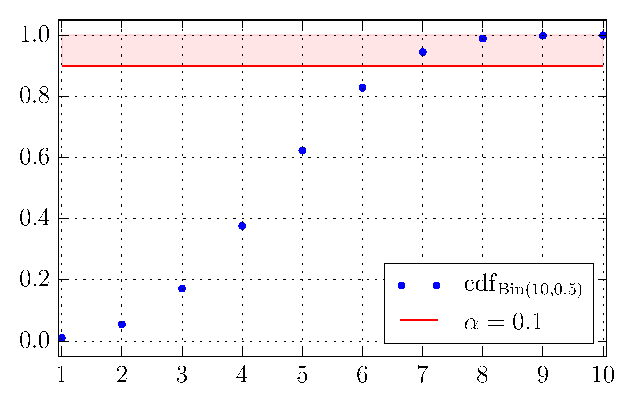
\includegraphics[width=0.5\textwidth]{fig/mouse-bin-cdf}
%\end{figure}
%
%
%\end{itemize}
%\end{example*}

%\section{Понятие гипотезы и критерия}
%
%Пусть $x_{1},\ldots,x_{n}\sim\Pcal$, $\Pscr$ --- множество всех
%распределений. О $\Pcal$ возможно делать утверждения вида $\Pcal\in\Pscr'\subset\Pscr$.
%Стоит задача выбрать такое утверждение, что оно некоторым наилучшим
%образом соответствует выборке.
%\begin{defn*}
%\emph{Модель} --- это предположение о выделенном классе $\Pscr_{M}\subset\Pscr$,
%которому принадлежит $\Pcal$ (допустим, $\Pscr_{M}=\left\{ \N({a},\sigma_{0})\right\} $,
%где $\sigma_{0}$ --- фиксированное значение). Иными словами, это
%утверждение о $\Pcal$, которое считается верным и не проверяется.
%\end{defn*}
%
%\begin{defn*}
%\emph{Гипотеза} --- утверждение о $\Pcal$, требующее проверки. Гипотеза
%называется \emph{простой}, если она соответствует только одному распределению
%в рамках рассматриваемой модели:
%\[
%H:\Pcal=\Pcal_{0}\in\Pscr_{M}
%\]
% (например, $\Pcal_{0}=\N({a}_{0},\sigma_{0})$) или \emph{сложной},
%если целому множеству:
%\[
%H:\Pcal\in\Pscr'\subset\Pscr_{M}
%\]
% (например, $\Pscr'=\left\{ \N({a},\sigma_{0}):{a}>0\right\} $).
%\end{defn*}
%Очень часто возникает (и далее рассматривается) случай выдвижения
%только лишь двух гипотез: $H_{0}:\Pcal\in\Pscr_{0}\subset\Pscr$ ---
%\emph{нулевой}, основной и $H_{1}:\Pcal\in\Pscr_{1}\subset\Pscr$
%--- \emph{альтернативной}. $H_{1}$ учитывает отклонения от $H_{0}$,
%обнаружение которых желательно. Возможны варианты:
%\begin{itemize}
%\item простая $H_{0}$ и простая $H_{1}$;
%\item простая $H_{0}$ и сложная $H_{1}$;
%\item сложная $H_{0}$ и сложная $H_{1}$.\end{itemize}
%\begin{defn*}
%\emph{Критерий} есть отображение
%\[
%\varphi:\mathbf{x}\mapsto\left\{ H_{0},H_{1}\right\} .
%\]
%
%\end{defn*}
%Критерий <<решает>>, противоречат или не противоречат выдвинутой
%гипотезе выборочные данные.
%\begin{defn*}
%Говорят, что гипотеза \emph{отвергается}, если $\varphi(\mathbf{x})=H_{1}$
%и \emph{не отвергается} иначе.
%\end{defn*}
%Так как в заданной постановке любой критерий принимает не более двух
%значений, то $\dom\varphi$ разбивается на два дизъюнктных множества
%$\Ascr_{\text{крит}}$ и $\Ascr_{\text{дов}}$, называемых
%\emph{критической} и \emph{доверительной} областями, таких, что
%\[
%\varphi(\mathbf{x})=\begin{cases}
%H_{0} & \mathbf{x}\in\Ascr_{\text{дов}}\\
%H_{1} & \mathbf{x}\in\Ascr_{\text{крит}.}
%\end{cases}
%\]
%
%
%Поскольку выборка конечного объема позволяет делать только вероятностные
%заключения, со статистическим критерием ассоциированы ошибки $i$-ых
%родов.
%\begin{defn*}
%Говорят, что произошла \emph{ошибка $i$-го рода} критерия $\varphi$,
%если критерий отверг верную гипотезу $H_{i-1}$. Соответствующие вероятности
%обозначаются
%\[
%\a_{i}(\varphi)=\P_{H_{i-1}}(\varphi(\mathbf{x})\neq H_{i-1}).
%\]
%
%
%Поскольку в рассмотрение введены только $H_{0}$ и $H_{1}$, возможны
%ошибки \emph{I-го рода} --- принятие случайного различия за систематическое
%и \emph{II-го рода} --- принятие наблюдаемого различия за случайный
%эффект с соответствующими вероятностями
%\begin{eqnarray*}
%\a_{\I} & = & \P_{H_{0}}(\varphi(\mathbf{x})\neq H_{0})=\P_{H_{0}}(\mathbf{x}\in\Ascr_{\text{крит}})\\
%\a_{\II} & = & \P_{H_{1}}(\varphi(\mathbf{x})\neq H_{1})=\P_{H_{1}}(\mathbf{x}\in\Ascr_{\text{дов}}).
%\end{eqnarray*}
%\end{defn*}
%\begin{rem*}
%Если $H_{i}$ --- сложная гипотеза, то $\a_{i+1}(\varphi)$ будет
%зависеть от того, на каком именно распределении $\Pcal$, отвечающем
%$H_{i}$, вычисляется эта вероятность.
%\end{rem*}
%
%\begin{defn*}
%\emph{Мощность} критерия против альтернативы это вероятность справедливо
%отвергнуть $H_{0}$:
%\[
%\b=1-\a_{\mathrm{II}}=1-\P_{H_{1}}(\varphi(\mathbf{x})=H_{0})=\P_{H_{1}}(\varphi(\mathbf{x})=H_{1}).
%\]
% Иными словами, это способность критерия отличать $H_{0}$ от $H_{1}$.
%\end{defn*}
%
%\section{Построение оптимальных критериев}
%
%Рассмотрим пример.
%\begin{example*}
%\label{exa:phi-b}Пусть $\xi\sim\N({a},1)$ и $\mathbf{x}=\left\{ x\right\} $.
%Выдвинем $H_{0}:{a}=0$ против простой альтернативы $H_{1}:{a}=1$
%Рассмотрим критерий
%\[
%\varphi_{b}(\mathbf{x})=\begin{cases}
%H_{0} & x<b\\
%H_{1} & x\geq b.
%\end{cases}
%\]
%(FIXME: Рисунок) Ясно, что из всего множества критериев $\left\{ \varphi_{b}\right\} $,
%не все одинаково хорошо описывают нормальную выборку: так, тождественный
%$\varphi_{\infty}(\mathbf{x})\equiv H_{0}$ будет вести себя хуже
%любого $\varphi_{b},\ b<\infty$.
%\end{example*}
%Выбирать оптимальный критерий можно тремя способами: минимаксным,
%Байесовским подходами и выбором наиболее мощного критерия.
%\begin{defn*}
%$\varphi^{(1)}$ не хуже $\varphi^{(1)}$ в \emph{минимаксном} смысле,
%если
%\[
%\max(\a_{\I}(\varphi^{(1)}),\a_{\II}(\varphi^{(1)}))\leq\max(\a_{\I}(\varphi^{(2)}),\a_{\II}(\varphi^{(2)})).
%\]
%Если $\phi^{*}$ не хуже всех остальных в этом смысле, то он называется
%\emph{минимаксным}.\end{defn*}
%\begin{example*}
%$\varphi_{1/2}$ минимаксный.\end{example*}
%\begin{defn*}
%Пусть известны $r=\P(H_{0})$, $s=1-r=\P(H_{1})$ (или задана линейная
%функция потерь, равная $r$ в случае ошибки 1-го рода и $s$ --- второго).
%Тогда $\varphi^{(1)}$ не хуже $\varphi^{(1)}$ в \emph{байесовском}
%смысле, если
%\[
%r\a_{\I}(\varphi^{(1)})+s\a_{\II}(\varphi^{(1)})\leq r\a_{\I}(\varphi^{(2)})+s\a_{\II}(\varphi^{(2)}).
%\]
%Если $\phi^{*}$ не хуже всех остальных в этом смысле, то он называется
%\emph{байесовским}.\end{defn*}
%\begin{rem*}
%Короче говоря, по правилу полной вероятности это вероятность ошибки
%критерия:
%\[
%\P(H_{0})\P(\underbrace{\varphi(\mathbf{x})=H_{1}}_{\mathrm{Err}}\mid H_{0})+\P(H_{1})\P(\underbrace{\varphi(\mathbf{x})=H_{0}}_{\mathrm{Err}}\mid H_{1})=\P(\mathrm{Err}).
%\]
%\end{rem*}
%\begin{example*}
%$\varphi_{1/2}$ байесовский с $s=r$.\end{example*}
%\begin{defn*}
%Пусть до эксперимента зафиксирован \emph{уровень значимости}\footnote{Неформально, $\a$ обратно пропорциональна <<строгости>> критерия,
%выбираемой экспериментатором.} критерия $\a\in\left[0,1\right]$. Критерий
%\[
%\varphi^{*}\in K_{\a}=\left\{ \varphi(\mathbf{x})\mid\a_{\I}(\varphi)\leq\a\right\}
%\]
% называется \emph{наиболее мощным} критерием, если
%\[
%\a_{\II}(\varphi^{*})\leq\a_{\II}(\varphi),\quad\forall\phi\in K_{\a}.
%\]
%\end{defn*}
%\begin{rem*}
%Стандартные уровни значимости: $\a=0.05$ или $\a=0.01$.
%\end{rem*}
%Все три подхода могут быть сведены к универсальному критерию --- критерию
%отношения правдоподобия.
%
%В примере \ref{exa:phi-b} интуитивно ясно, что следует выбрать ту
%гипотезу, значение плотности которой в точке $x$ больше другой. В
%случае, если $n>1$, справедливо взять произведение плотностей ---
%т.е. функций правдоподобия и рассматривать их отношение
%\[
%L(\mathbf{x})=\frac{\L_{2}(\thb\mid\mathbf{x})}{\L_{1}(\thb\mid\mathbf{x})}.
%\]
%Выбор гипотезы затем делать по тому, больше или меньше $L$ единицы.
%Однако, чтобы учесть произвольный уровень ошибки, следует сравнивать
%не с 1, а с константой $c$.
%\begin{defn*}
%Пусть $\Pcal_{0},\Pcal_{1}$ либо одновременно дискретны, либо непрерывны.
%Пусть также $\neg\exists c_{0}:\P_{H_{0}}(L(\mathbf{x})=c_{0})=0$
%(в противном случае критерий не сможет различить гипотезы на множестве
%не-нулевой меры) --- т.е., $\P_{H_{0}}(L(\mathbf{x})\geq c)$ непрерывна
%по $c>0$. Тогда \emph{критерием отношения правдоподобия} называется
%\[
%\varphi_{c}(\mathbf{x})=\begin{cases}
%H_{0} & L(\mathbf{x})<c\\
%H_{1} & L(\mathbf{x})\geq c.
%\end{cases}
%\]
%
%\end{defn*}
%
%\subsection{Явный вид оптимальных критериев}
%\begin{claim*}
%В предположениях из определения, критерий отношения правдоподобия
%является
%\begin{enumerate}
%\item минимаксным при $c:\a_{\I}(\varphi_{c})=\a_{\II}(\varphi_{c})$;
%\item байесовским при заданных $r,s:c=r/s$;
%\item (лемма Неймана-Пирсона) наибольшей мощности при заданном $\a:\a_{\I}(\varphi_{c})=\a.$
%\end{enumerate}
%\end{claim*}
%\begin{example*}
%Пусть $\xi\sim\N({a},1)$. $H_{0}:{a}={a}_{0}$, $H_{1}:{a}={a}_{1}>{a}_{0}$.
%Критическая область задается неравенством
%\[
%L(\mathbf{x})=\frac{\L_{2}(\thb\mid\mathbf{x})}{\L_{1}(\thb\mid\mathbf{x})}=\exp\left(\frac{1}{2\sigma^{2}}\sum_{i=1}^{n}\left(x_{i}-{a}_{0}\right)^{2}-\left(x_{i}-{a}_{1}\right)^{2}\right)\geq c,
%\]
%упрощая которое получают
%\[
%\bar{x}\geq\frac{\ln c}{({a}_{1}-{a}_{0})n}+\frac{{a}_{1}-{a}_{0}}{2}.
%\]
%
%\begin{itemize}
%\item Пусть критерий байесовский с $r=1/4$, $s=3/4$; тогда $c=1/3$.
%\item Пусть критерий наибольшей мощности c заданным $\a$, критическая область
%задается $\bar{x}\geq c_{0}.$ Тогда
%\[
%\a_{\I}=\P_{H_{0}}(\bar{x}\geq c_{0})=\P_{H_{0}}(\sqrt{n}(\bar{x}-{a}_{0})\geq\sqrt{n}\left(c_{0}-{a}_{0}\right))=1-\cdf_{\N(0,1)}\left(\sqrt{n}\left(c_{0}-{a}_{0}\right)\right)=\a
%\]
%если
%\[
%c_{0}=\frac{z_{1-\a}}{\sqrt{n}}+{a}_{0}.
%\]
%
%\item Пусть критерий минимаксный. Тогда
%\[
%\a_{\II}=\cdf_{\N(0,1)}\left(\sqrt{n}(c_{0}-{a}_{1})\right)=1-\cdf_{\N(0,1)}(\sqrt{n}(c_{0}-{a}_{0}))=\cdf_{\N(0,1)}(\sqrt{n}({a}_{0}-c_{0}))
%\]
% если
%\[
%c_{0}-{a}_{1}={a}_{0}-c_{0},\quad c_{0}=\frac{{a}_{0}+{a}_{1}}{2}.
%\]
%
%\end{itemize}
%\end{example*}
%\begin{defn*}
%Критерий называется \emph{состоятельным }против альтернативы $H_{1}$,
%если $\forall\Pcal_{1}\in\Pscr_{1}$
%\[
%\b(\varphi,\Pcal_{1})=1-\P_{\Pcal_{1}}(\varphi(\mathbf{x})=H_{0})\xrightarrow[n\to\infty]{}1.
%\]
%\end{defn*}
%\begin{example*}
%Критерий наибольшей мощности
%\[
%\varphi(\mathbf{x})=\begin{cases}
%H_{0} & \bar{x}<\frac{z_{1-\a}}{\sqrt{n}}+{a}_{0}\\
%H_{1} & \text{иначе}
%\end{cases}
%\]
% является состоятельным, потому что
%\[
%\a_{\II}(\varphi)=\P_{H_{1}}\left(\bar{x}-\frac{z_{1-\a}}{\sqrt{n}}<{a}_{0}\right),
%\]
% но, при верной $H_{1}$,
%\[
%\xi_{n}=\bar{x}-\frac{z_{1-\a}}{\sqrt{n}}\toP{a}_{1},
%\]
% из чего следует слабая сходимость --- сходимость $\cdf_{\xi_{n}}(x)\to\cdf_{{a}_{1}}(x)=\P({a}_{1}<x)$
%по всех точках; учитывая $\cdf_{{a}_{1}}({a}_{0})=0$,
%\[
%\a_{\II}(\varphi)=F_{\xi_{n}}({a}_{0})\to F_{{a}_{1}}({a}_{0})=0.
%\]
%
%\end{example*}
%
%\begin{defn*}
%Если
%\begin{labeling}{00.00.0000}
%\item [{$\a_{\I}=\a$}] то критерий называется \emph{точным},
%\item [{$\a_{\I}\xrightarrow[n\to\infty]{}\a$}] \emph{асимптотическим},
%\item [{$\a_{\I}>\a$}] \emph{радикальным} (т.е. отвергает гипотезу чаще,
%чем точный),
%\item [{$\a_{\I}<\a$}] \emph{консервативным} (если гипотеза отвергнута,
%то уж наверняка).
%\end{labeling}
%\end{defn*}
%
%
%
%\subsection{О постановке $H_{0}$}
%
%\label{rem:form-h0}Задача может допускать две постановки; в этом
%случае, поскольку $\a_{\I}$ ($=\a$ для правильно построенного критерия)
%контролируется экспериментатором, проверяется отрицание эффекта, который
%хотят подтвердить: к примеру, что новое лекарство \emph{не} лучше
%старого; если $H_{0}$ отвергнется, это будет означать, что новое
%лекарство-таки лучше старого с вероятностью не ниже, чем $1-\a$.
%
%\begin{comment}
%Некто заявляет о способности не глядя угадывать масти предлагаемых
%карт. Выдвигаем гипотезу $H_{0}$: человек \emph{не} экстрасенс, так
%что угадывает с вероятностью $p=1/4$. Предлагаем отгадать масть 25
%карт; число угаданных карт есть $x$. Наибольшей <<строгости>> будет
%соответствовать $x=25$, таким образом
%\[
%\P_{H_{0}}(x\in\Ascr_{\text{крит}})=\P_{H_{0}}(x=25)=\left(\frac{1}{4}\right)^{25}\approx10^{-15}=\a.
%\]
% Если же для нас достаточно 24 угаданных карт из 25, то $\a$ будет
%побольше: $\P_{H_{0}}(x\geq24)=\P_{H_{0}}(x=24)+\P_{H_{0}}(x=25)$
%и т.д. Зафиксированная до эксперимента $\a$ определяет количество
%карт $c$ такое, что при угадывании большего количества $H_{0}$ будет
%считаться опровергнутой:
%\[
%\a_{\I}=\P_{H_{0}}(x\geq c)\leq\a.
%\]
% Среди всех таких $c$ следует выбрать наименьшее, чтобы минимизировать
%ошибку второго рода.
%\end{comment}
%\begin{comment}
%@xio: TODO: дописать, почему.
%\end{comment}
%\begin{comment}
%@xio: нельзя ли сказать, что в этом случае использовалась простая
%статистика --- количество угаданных карт?
%\end{comment}
%
%\begin{example*}[С гранатами]
%\begin{comment}
%@xio: FIXME
%\end{comment}
%FIXME
%\end{example*}
%
%\subsection{Об отвержении гипотезы}
%
%Утверждать об \emph{отвержении} гипотезы можно с вероятностью ошибки
%$\a$ (достаточно малой и произвольно задаваемой экспериментатором);
%утверждать о \emph{принятии} гипотезы можно с вероятностью ошибки
%$\a_{\mathrm{II}}$ --- не контролируемой и потенциально довольно
%большой. Иными словами, попадание в доверительную область может означать
%как то, что $H_{0}$ верна, так и то, что верна $H_{1}$, но для распознания
%этого не хватило мощности. Поэтому безопасно гипотезу можно только
%отвергать или не отвергать. Можно и принять, если известна мощность
%критерия против всех возможных альтернатив, экспериментатора устраивающая.
%
%При высокой вероятности ошибки II-го рода возможна ситуация не отвержении
%заведомо ложной гипотезы. Это, в свою очередь, может произойти из-за
%маленького объема выборки (критерий не находит разницу, см. \ref{exa:h0-h1}).
%Чем больше объем выборки, тем мощность больше, но возможна ситуация,
%когда критерий чувствителен настолько, что находит разницу там, где
%не должен --- например, при генерации <<идеальным>> датчиком случайных
%чисел, начиная с какого-то объема заведомо истинная гипотеза может
%быть отвергнута из-за ошибок в точности представления чисел с плавающей
%точкой.
%\begin{defn*}
%\emph{Критерий} называется \emph{одно- (двух-) сторонним} по тому,
%где находится альтернатива.
%\end{defn*}
%
%\begin{defn*}
%\emph{Критическая область} называется \emph{одно- (дву-) сторонней
%}по тому, где формально располагается $\Ascr_{\text{крит}}$.
%\end{defn*}

%\section{Построение критерия при помощи статистики критерия}
%\begin{defn*}
%\emph{Статистика критерия} есть отображение
%\[
%T:\mathbf{x}\mapsto y\in\RR
%\]
% такое, что при верной $H_{0}$, $T\tod\mathcal{Q}$, где $\mathcal{Q}$
%--- полностью известное непрерывное распределение, а при верной $H_{1}$
%известно поведение $T$.
%\end{defn*}
%Поскольку распределение $T$ при верной $H_{0}$ известно, она должна
%вести себя как любая другая случайная величина из $\mathcal{Q}$ ---
%попадание в некоторые области менее вероятно, чем в другие. Поэтому
%разумно разбить $\supp T$ по уровню значимости $\a$ на $\Ascr_{\text{крит}}\sqcup\Ascr_{\text{дов}}$
%так, что попадание в $\Ascr_{\text{крит}}$ \emph{при верной $H_{0}$}
%происходит с заранее зафиксированной (малой) вероятностью $\a$. Значит,
%если $T(\mathbf{x})\in\Ascr_{\text{крит}}$, то с некоторой же
%вероятностью можно заявлять об отвержении $H_{0}$. Таким образом,
%$T$ измеряет то, насколько выборка соответствует гипотезе.
%
%
%\section{Разбиение на доверительную и критические области}
%
%Разберем на примере построение разбиения. Пусть $\xi\sim\N({a},\sigma^{2})$,
%$H_{0}:{a}={a}_{0}$ и фиксирован $\a$.
%Используется статистика
%\[
%t=z=\sqrt{n}\frac{\bar{x}-a_{0}}{\sigma}\sim\N(0,1).
%\]
%В зависимости от $H_{1}$, возможны варианты.
%
%
%\subsection{Простая альтернатива}
%
%\label{exa:h0-h1}Пусть $H_{1}:{a}={a}_{1}$, причем ${a}_{1}>{a}_{0}$.
%Тогда, поскольку при верной $H_{1}$, $\E\bar{x}=1/n\cdot\sum_{i=1}^{n}\xi_{i}=n/n\cdot{a}_{1}$,
%то
%\[
%\E T=\frac{\sqrt{n}\left({a}_{1}-{a}_{0}\right)}{\sigma}\implies T\sim\N\left(\frac{\sqrt{n}\left({a}_{1}-{a}_{0}\right)}{\sigma},1\right)\text{ при верной }H_{1}.
%\]
%(дисперсия, конечно, не меняется при сдвиге).
%
%\begin{figure}[H]
%\centering{}\includegraphics[width=0.5\textwidth]{fig/h0_h1}\caption{Плотности распределения $z$ (неоптимальное разбиение)}
%\end{figure}
%
%
%Чтобы минимизировать $\a_{\mathrm{II}}$, логично определить $\Ascr_{\text{крит}}$
%только на одном хвосте --- с той стороны, где находится альтернатива.
%Помимо этого, по рисунку видно, что минимизировать $\a_{\mathrm{II}}$
%(согласившись на б\'oльшую ошибку первого рода) можно сдвинув вправо
%центр второй плотности, увеличив $n$. Аналогично, чем ${a}_{1}$
%дальше от ${a}_{0}$, тем $\a_{\mathrm{II}}$ меньше.
%
%\begin{figure}[H]
%\centering{}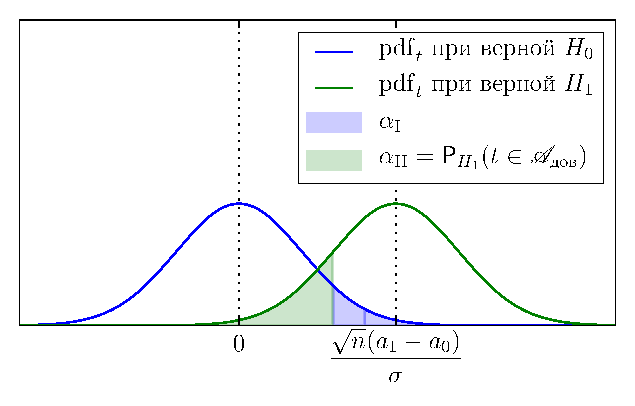
\includegraphics[width=0.5\textwidth]{fig/h0_h1-opt}\caption{Плотности распределения $z$ (оптимальное разбиение)}
%\end{figure}
%
%
%Таким образом, $\Ascr_{\text{крит}}=(C,+\infty)$, $C=z_{1-\a}$.
%
%Разумеется, если ${a}_{_{1}}<{a}_{0}$, то $\Ascr_{\text{крит}}=(-\infty,C),$
%$C=z_{\a}$.
%
%
%\subsection{Односторонний критерий (сложная альтернатива)}
%
%В общем случае, пусть $H_{1}:{a}={a}_{1}\ \forall{a}_{1}>{a}_{0}$;
%тогда по ЗБЧ $\bar{x}-{a}_{0}\to{a}_{1}-{a}_{0}>0$ и $T\to+\infty$.
%Следовательно, чтобы максимизировать величину $\b=\P_{H_{1}}(\mathbf{x}\in\Ascr_{\text{крит}}^{(\a)}),$
%следует разместить $\Ascr$ на правом хвосте плотности: $\Ascr_{\text{крит}}=\left(z_{1-\a},\infty\right)$.
%Для $H_{1}:{a}={a}_{1}\ \forall{a}_{1}<{a}_{0}$ аналогично $\Ascr_{\text{крит}}=\left(-\infty,z_{\a}\right)$.
%
%
%\subsection{Двусторонний критерий}
%
%\begin{comment}
%В случае $T\sim\N(0,1)$, разумно определить $\Ascr_{\text{крит}}$
%<<на хвостах>> графика $\pdf_{\N(0,1)}$ симметрично по обе стороны
%от 0 так, что для $\Ascr_{\text{крит}}=(-\infty,T_{0})\cup(T_{1},\infty)$
%\[
%\a/2=\int_{-\infty}^{T_{0}}\pdf_{\N(0,1)}(y)\d y=\int_{T_{1}}^{+\infty}\pdf_{\N(0,1)}(y)\d y.
%\]
% Иными словами,
%\[
%\a/2=1-\cdf_{\N(0,1)}(T_{1})\implies T_{1}=\cdf_{\N(0,1)}^{-1}(1-\a/2)
%\]
%и аналогично для $T_{0}$.
%\end{comment}
%Пусть $H_{1}:\E\xi={a}_{1}\neq{a}_{0}$; тогда по ЗБЧ $\bar{x}-{a}_{0}\to{a}_{1}-{a}_{0}$
%и $\left|T\right|\xrightarrow[n\to\infty]{}\infty$, откуда $\Ascr_{\text{крит}}=\RR\setminus\left(z_{\a/2},z_{1-\a/2}\right)=\RR\setminus\left(-C,C\right)$,
%где $C=-z_{\a/2}$.
%
%В общем виде, с использованием статистики, критерий может быть определен
%как
%\[
%\varphi(\mathbf{x})=\begin{cases}
%H_{0} & \left|T(\mathbf{x})\right|<C\\
%H_{1} & \left|T(\mathbf{x})\right|\geq C,
%\end{cases}
%\]
%где \emph{критическое значение} $C$ определяется из уравнения $\a=\P(\left|T\right|\geq C)$.
%
%Иногда вместо сравнения значения $T$ с критическим вычисляют \emph{реально
%достигнутый уровень значимости критерия} (<<\emph{$p$-value}>>).
%\begin{defn*}
%\emph{$p$-value }значения статистики $T$ на выборке $\mathbf{x}$
%есть вероятность, взяв выборку из распределения $H_{0}$, получить
%по ней большее отклонение $\left|T(\mathbf{x})\right|$ эмпирического
%от истинного распределения, чем получено по проверяемой выборке:
%\[
%\pv=\a^{*}=\P_{H_{0}}(\left|T\right|\geq\left|T(\mathbf{x})\right|).
%\]
%\begin{comment}
%@xio: TODO: картина с bellcurve, $t_{\mathrm{obs}}$ пойнтом и закрашенной
%вероятностью справа от нее.
%\end{comment}
%
%\end{defn*}
%Значит, критерий может быть задан и как
%\[
%\varphi(\mathbf{x})=\begin{cases}
%H_{0} & \a^{*}>\a\\
%H_{1} & \a^{*}\leq\a.
%\end{cases}
%\]
%
%\begin{rem*}
%$p$-value обратно пропорционален <<существенности>> результата.%
%\begin{comment}
%Иными словами, это мера согласованности $H_{0}$ и выборки.
%\end{comment}
%
%\end{rem*}
%
%\begin{rem*}
%Пусть $\a^{*}=0.05$. Это значит, что в среднем всего лишь 5\% <<контрольных>>
%выборок, удовлетворяющих основной гипотезе, будут обладать большим
%отклонением $\left|T(\mathbf{x})\right|$ по сравнению с тестируемой
%выборкой --- последняя ведет себя не хуже, чем 5\% <<правильных>>
%выборок.
%\end{rem*}
%
%\section{Схема построения критерия с помощью статистики }
%\begin{enumerate}
%\item Фиксируют предположение относительно данных.
%\item Выдвигают $H_{0}$ и $H_{1}$.
%
%\begin{itemize}
%\item $H_{0}$ формулируется согласно замечанию \ref{rem:form-h0}.
%\item $H_{1}$ ставится по смыслу задачи (см. далее).
%\end{itemize}
%\item Выбирают подходящий критерий и статистику $T$.
%\item Фиксируют уровень значимости $\a$.
%\item Строят разбиение $\im T$ с помощью квантилей распределения $T$ (при
%верной $H_{0}$) так, чтобы $\a_{\I}=\a$; положение квантилей выбирают
%из известного поведения статистики при верной $H_{1}$.
%\item Считают значение статистики и принимают решение об отвержении $H_{0}$
%одним из способов:
%\[
%\varphi(\mathbf{x})=\begin{cases}
%H_{0} & \left|T(\mathbf{x})\right|<C\\
%H_{1} & \left|T(\mathbf{x})\right|\geq C,
%\end{cases}\qquad\varphi(\mathbf{x})=\begin{cases}
%H_{0} & \a^{*}>\a\\
%H_{1} & \a^{*}\leq\a.
%\end{cases}
%\]
%\end{enumerate}
%\begin{example*}[Средняя температура в холодильнике]
%Хотят купить холодильник, такой, чтобы температура держалась в окрестности
%0. Известно количество измерений $n=25$ и $\bar{x}=0.7$.
%\begin{enumerate}
%\item Пусть $\xi\sim\N({a},4)$.
%\item Выдвинута $H_{0}:\E\xi={a}_{0}=0$ --- если гипотеза опровергнется,
%то холодильник не купят; $H_{1}:\E\xi={a}_{1}\neq{a}_{0}$.
%\item Поскольку модель нормальная и известная $\sigma^{2}$, выберем статистику
%\ref{sub:E_xi_norm} (<<z-test>>):
%\[
%z=\dfrac{\sqrt{n}\left(\bar{x}-{a}_{0}\right)}{\sigma}\sim\N(0,1)\text{ при верной }H_{0}.
%\]
% Идеальное значение статистики --- 0.
%\item Зафиксируем два уровня значимости: $\a^{(1)}=0.2$ (храним петрушку)
%и $\a^{(2)}=0.01$ (храним дорогую красную икру).
%\item Построим разбиение. Поскольку ${a}_{1}\neq{a}_{0}$, то $\Ascr_{\text{крит}}=\RR\setminus(z_{\a/2},z_{1-\a/2})$.
%Для введенных уровней значимости это означает
%
%\begin{enumerate}
%\item $\Ascr_{\text{крит}}^{(\a^{(1)})}\approx\RR\setminus\left(-1.28,1.28\right)$.
%\item $\Ascr_{\text{крит}}^{(\a^{(2)})}\approx\RR\setminus\left(-2.576,2.576\right)$.
%\end{enumerate}
%\item Посчитаем
%\[
%z(\mathbf{x})=\dfrac{\sqrt{n}\left(\bar{x}-{a}_{0}\right)}{\sigma}=\frac{5(0.7-0)}{2}=1.75.
%\]
%Дальнейшее принятие решения возможно на основании критического значения
%или $p$-value.
%
%\begin{itemize}
%\item По вычислению критического значения:
%
%\begin{itemize}
%\item $z\in\Ascr_{\text{крит}}^{(\a^{(1)})}$, $H_{0}$ отвергается,
%холодильник не покупают.
%\item $z\in\Ascr_{\text{дов}}^{(\a^{(2)})}$, $H_{0}$ не отвергается,
%холодильник, быть может, покупают.
%\end{itemize}
%\item Можно посчитать $p$-value:
%\[
%2\cdot(1-\cdf_{\N(0,1)}(1.75))\approx0.08.
%\]
% Поэтому при уровне значимости $\a^{(1)}=0.2>0.08$ $H_{0}$ отвергается,
%а при $\a^{(2)}=0.01<0.08$ не отвергается.
%\end{itemize}
%\end{enumerate}
%\end{example*}
%
%\begin{example*}[С мышой]
%В одном из рукавов T-образного лабиринта лежит морковка. К развилке
%по лабиринту бежит мышь и 7 раз из 10 поворачивает в направлении морковки.
%На основании этих данных хотим сделать вывод, что мышь чует морковь
%на расстоянии, после чего написать научную статью.
%\begin{itemize}
%\item $\xi\sim\Ber(p)$. Выдвинем гипотезу, что мышь \emph{не} чует морковку,
%$H_{0}:p=p_{0}=0.5$. Поскольку $\E\xi=p$, воспользуемся критерием
%для проверки гипотезы о значении среднего с идеальным значением 0;
%учитывая $\D\xi=p(1-p)$,
%\begin{eqnarray*}
%T & = & \sqrt{n}\frac{\bar{x}-p_{0}}{\sqrt{p_{0}(1-p_{0})}}\tod\N(0,1).\\
% & = & \frac{\sqrt{10}\cdot0.2}{0.5}\approx1.2649\implies p\text{-value}=2\cdot(1-\cdf_{\N(0,1)}(1.2649))\approx0.2.
%\end{eqnarray*}
% Значит, с уровнем значимости $0.2$ гипотеза не отвергается. Хочется
%иметь, конечно, один из стандартных уровней значимости, например $0.1$.
%\item Увеличим мощность критерия, введя альтернативную гипотезу, что мышь
%чует морковку (в предположении, что все мыши любят морковь и к ней
%бегут), $H_{1}:p_{1}>p_{0}$. По \ref{exa:h0-h1}, можем устроить
%односторонний критерий, так что $p$-value теперь 0.1. Однако пользуемся
%асимптотическим критерием при $n=10$.
%\item Воспользуемся точным односторонним критерием со статистикой
%\[
%T:=n\bar{x}=\sum_{i=1}^{n}x_{i}\sim\Bin(n,p_{0})
%\]
% и идеальным значением $np_{0}$. Тогда $T=10\cdot0.7=7$. При уровне
%значимости $\a=0.1$ успешно попадаем в критическую область, вследствие
%чего $H_{0}$ отвергается, и можем публиковаться.
%
%
%\begin{figure}[H]
%\centering{}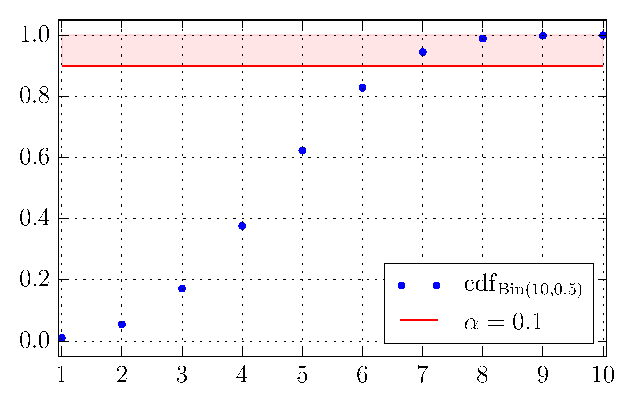
\includegraphics[width=0.5\textwidth]{fig/mouse-bin-cdf}
%\end{figure}
%
%
%\end{itemize}
%\end{example*}
%\begin{rem*}
%Исторически существовало два подхода к проверке гипотез: Фишера (<<significance
%test>>) и Неймана-Пирсона (<<hypothesis testing>>).
%\begin{description}
%\item [{Фишер}] Выдвигается $H_{0}$. Подсчитывается и сообщается точное
%$p$-value. Если результат <<незначительный>>, не делается никаких
%выводов об отвержении $H_{0}$, но делается возможным дополнительный
%сбор данных.
%\item [{Нейман-Пирсон}] Выдвигаются $H_{1},H_{2}$, фиксируются $\a_{\I},\a_{\II}$
%и $n$. На этом основании определяются $\Ascr_{\text{крит}}$
%для каждой гипотезы. Если данные попали в $\Ascr_{\text{крит}}$
%$H_{1}$ --- предпочитается $H_{2}$, иначе $H_{2}$.
%\end{description}
%Современная теория проверки гипотез есть смесь двух этих подходов,
%не всегда консистентная. Вводные курсы по статистике формулируют теорию,
%похожую на significance testing Фишера; при повышенных требованиях
%к математической строгости, пользуются теорией Неймана-Пирсона.
%\end{rem*}
%
%\begin{rem*}[О графике $p$-values]
%Поскольку
%\[
%\a_{\mathrm{I}}\gets\P_{H_{0}}(T\in\Ascr_{\text{крит}})=\P_{H_{0}}(p\text{-value}<\a),
%\]
%то $p$-value по распределению стремятся к $\U(0,1)$ при верной $H_{0}$.
%Это соображение позволяет визуально проверить истинность гипотезы:
%достаточно несколько (много) раз произвести эксперимент, для каждой
%выборки $\bar{x}^{(i)}$ посчитать свой $p$-value, построить
%график и убедиться, что получилась прямая. %
%\begin{comment}
%@xio: проверить
%\end{comment}
%{} Для подсчета мощности $\b=\P_{H_{1}}(\mathbf{x}\in\Ascr_{\text{крит}}^{(\a)})=\P_{H_{1}}(p\text{-value}<\a)$
%считать выборку с параметрами $H_{1}$, а $T$ относительно $H_{0}$.
%\end{rem*}

\end{document}
\chapter{Проверка гипотезы о значении параметра (характеристики)}

\section{Проверка гипотезы о значении мат. ожидания ($t$-критерий)}
\label{sec:ttest}
$H_{0}:\E\xi={a}={a}_{0}$. Соответствие оценки математического ожидания
гипотезе удобно выражать разницей $\bar{x}-{a}_{0}$ с <<идеальным>>
значением 0. Отнормировав эту разницу, получим статистику, распределение
которой известно.


\subsection{$\protect\D\xi=\sigma^{2}<\infty$}
\begin{prop*}
Пусть $\D\xi=\sigma^{2}<\infty$; тогда используется следующая статистика ($z$-score)
\[
t=z=\sqrt{n}\frac{(\bar{x}-{a}_{0})}{\sigma}\xrightarrow[n\to\infty]{}\N(0,1)
\]
 \end{prop*}
\begin{prop*}
При условии $\xi\sim \N(a,\sigma^2)$,
\[
t=z\sim\N(0,1).
\]
\end{prop*}
\begin{proof}
\[
z=\frac{\bar{x}-{a}_{0}}{\sqrt{\D\bar{x}}}=\sqrt{n}\,\dfrac{\bar{x}-{a}_{0}}{\sigma}\sim\N(0,1).
\]

\end{proof}

%\paragraph{Разбиение}
%\begin{description}
%\item [{$H_{1}:\E\xi\neq{a}_{0}$}] $\Ascr_{\text{крит}}=\RR\setminus\left(z_{\a/2},z_{1-\a/2}\right)$
%\item [{$H_{1}:\E\xi>{a}_{0}$}] $\Ascr_{\text{крит}}=(z_{1-\a},\infty)$
%\item [{$H_{1}:\E\xi<{a}_{0}$}] $\Ascr_{\text{крит}}=(-\infty,z_{\a})$
%\end{description}

\subsection{$\protect\D\xi$ неизвестна}
\label{sect:expect_gen}
\begin{prop*}
Пусть $\D\xi$ неизвестна; тогда используется следующая статистика
\[
t=\sqrt{n-1}\,\frac{\bar{x}-{a}_{0}}{s}=\sqrt{n}\,\frac{\bar{x}-{a}_{0}}{\tilde{s}}\xrightarrow[n\to\infty]{}\N(0,1).
\]
\end{prop*}


Сходимость к нормальному распределению следует из модифицированной теоремы Леви (модифицированная ЦПТ), которая позволяет заменять дисперсию на ее состоятельную оценку с сохранением сходимости к тому же нормальному распределению.


\begin{prop*}
В модели, когда $\xi$ имеет нормальное распределение,
\[
t\sim\t(n-1).
\]
\end{prop*}

\begin{comment}
\[
\sum_{i=1}^{n}(x_{i}-\E\xi)^{2}=\sum_{i=1}^{n}(x_{i}-\bar{x})^{2}+n(\bar{x}-\E\xi)^{2}
\]
 --- разложение кв. ф.
\end{comment}



%\paragraph{Разбиение}
%\begin{description}
%\item [{$H_{1}:\E\xi\neq{a}_{0}$}] $\Ascr_{\text{крит}}=\RR\setminus\left(\qnt_{\t(n-1)}(\a/2),\qnt_{\t(n-1)}(1-\a/2)\right)$
%\item [{$H_{1}:\E\xi>{a}_{0}$}] $\Ascr_{\text{крит}}=(\qnt_{\t(n-1)}(1-\a),\infty)$
%\item [{$H_{1}:\E\xi<{a}_{0}$}] $\Ascr_{\text{крит}}=(-\infty,\qnt_{\t(n-1)}\a)$\end{description}
%\begin{rem*}
%При нормальной аппроксимации $\qnt_{\t(n-1)}$ заменить на $\N(0,1)$.
%\end{rem*}

\subsection{Проверка гипотезы о мат.ож. в модели с одним параметром}
\label{sect:expect_one}

Разница с общим случаем состоит в том, что в параметрической модели с одним параметром не нужно оценивать дисперсию. Так как все выражается через этот параметр, то имеем формулу для дисперсии через значение параметра, предполагаемое в нулевой гипотезе.

\paragraph{$z$-критерий для пропорции в модели Бернулли}
Пусть $\xi\sim\Ber(p)$. Поскольку $\E\xi=p$, можно воспользоваться
только что введенной статистикой; учитывая $\D\xi=p(1-p)$, получаем статистику критерия для гипотезы $H_0: p=p_0$:
\[
t=\sqrt{n}\frac{\bar{x}-p_{0}}{\sqrt{p_{0}(1-p_{0})}}\tod\N(0,1).
\]

\paragraph{$z$-критерий для интенсивности потока в модели Пуассона}
Пусть $\xi\sim\Pois(\lambda)$. Поскольку $\E\xi=\lambda$, можно воспользоваться
только что введенной статистикой; учитывая $\D\xi=\lambda$, получаем статистику критерия для гипотезы $H_0: \lambda=\lambda_0$:
\[
t=\sqrt{n}\frac{\bar{x}-\lambda_{0}}{\sqrt{\lambda_{0}}}\tod\N(0,1).
\]

\section{Критерий $\chi^{2}$}

По выборке возможно проверить гипотезу о виде распределения случайной
величины, реализацией которой является выборка.
Для проверки гипотезы согласия с видом произвольного \emph{дискретного}
распределения используется асимптотический \emph{критерий $\chi^{2}$
(<<chi-squared test for goodness of fit>>).}

\subsection{Распределение с известными параметрами}

Пусть
\[
H_{0}:\Pcal=\Pcal_{0},\text{ где }\Pcal_{0}:\begin{pmatrix}x_{1}^{*} & \dots & x_{k}^{*}\\
p_{1} & \dots & p_{k}
\end{pmatrix}.
\]
 Сгруппируем $\mathbf{x}$; каждому $x_{i}^{*}$ сопоставим \emph{эмпирическую}
абсолютную частоту $\nu_{i}$; тогда $np_{i}$ --- \emph{ожидаемая}
абсолютная частота.

В качестве меры расхождения между эмпирическим и генеральным распределением
рассматривается величина
\[
\sum_{i=1}^{k}c_{i}\left(\frac{\nu_{i}}{n}-p_{i}\right)^{2},\quad c_{i}=\frac{n}{p_{i}},
\]
 откуда записывается статистика критерия
\[
T=\sum_{i=1}^{k}\frac{(\nu_{i}-np_{i})^{2}}{np_{i}}
\]
 с `идеальным' значением 0 (следовательно, критическая область только справа).
\begin{claim*}
$T\tod\chi^{2}(k-1)$.
\end{claim*}

%\paragraph{Разбиение}
%
%$\Ascr_{\text{крит}}=\left(\qnt_{\chi^{2}(k-1)}(1-\a),\infty\right)$
%--- гипотеза отвергается, если расстояние между предполагаемым и наблюдаемым
%распределениями большое.

\begin{defn*}
Критерий \emph{применим}, если $\a_{\mathrm{I}}=\a$ или $\a_{\mathrm{I}}\approx \a$ с достаточной степенью точности.%
\begin{comment}
@xio: так?
\end{comment}
\begin{comment}
$n\downarrow\implies$ не применим
\end{comment}
\end{defn*}
\begin{rem*}
Поскольку критерий асимптотический, с достаточной (тому, кто дает такие рекомендации) степенью точностью
он применим в случае, если
\begin{enumerate}
\item $n\geq50$;
\item $np_{i}\geq5.$
\end{enumerate}
\end{rem*}

\begin{rem*}
Если условие $np_{i}\geq5$ не выполняется, следует объединить состояния,
например, с краев или слева направо; если в хвосте оказалось $<5$,
то следует присоединить к последнему.\end{rem*}

\begin{rem*}
Почему бы не подстраховаться и не объединить состояния так, чтобы было >10? Ответ: теряем в мощности. \\
\textbf{Задание} Привести пример, демонстрирующий потерю мощности.
\end{rem*}


\begin{example*}[С монеткой]
Пусть $n=4040$, $\#\mathrm{H}=2048,\ \#\mathrm{T}=1092$. Проверим
$H_{0}:\Pcal=\Ber(0.5)$ с $\a=0.1$. Условия критерия выполняются,
поэтому посчитаем
\[
T=\frac{(2048-2020)^{2}}{2020}+\frac{(1092-2020)^{2}}{2020}=\frac{28^{2}+28^{2}}{2020}\approx0.78,
\]
откуда
\[
p\text{-value}=1-\cdf_{\chi^{2}(1)}(0.78)\approx0.38.
\]
 $0.38>0.1$, значит $H_{0}$ не отвергается.\end{example*}
\begin{rem*}
Если нужно подстраховаться от подгонки (искусственно составленных под гипотезу выборок), то критическую область можно выбрать с двух сторон, слева и справа. Например, чтобы отверглась гипотеза о $p=0.5$ для альтернирующей (и явно не
случайной) последовательности $\mathbf{x}=(0,1,0,1,\ldots)$ имеет
$T=0$.
Однако, если мы не подозреваем данные в обмане, то так не делают.
\begin{comment}
@xio: вставить про разные виды графиков: не случайная выборка ---
выгнута вверх, не равномерная --- вниз?
\end{comment}

\end{rem*}



%\begin{xca*}
%$n=100$,
%\[
%\begin{pmatrix}\diamondsuit & \heartsuit & \clubsuit & \spadesuit\\
%20 & 30 & 10 & 40
%\end{pmatrix}.
%\]
% Проверить гипотезу, что колода полная.\end{xca*}
%\begin{solution}
%$H_{0}:\Pcal_{\xi}=\U(1/4)$. Поскольку речь идет о согласии с дискретным
%не параметризованным распределением, напрямую воспользуемся критерием
%$\chi^{2}$. Раз все $np_{i}=100\cdot1/4=25,$
%\[
%\chi^{2}=\sum_{i=1}^{k}\frac{(\nu_{i}-np_{i})^{2}}{np_{i}}=1+1+\frac{15^{2}}{25}+\frac{15^{2}}{25}=2+2\cdot9=20.
%\]
% Так как $\chi^{2}\sim\chi^{2}(k-1)=\chi^{2}(3)$ со средним 3, и
%<<идеальное>> значение 0, определим критическую область в правом
%конце плотности. Из этих соображений
%\[
%\pv=1-\cdf_{\chi^{2}(3)}(20)=1-\mathtt{pchisq(20,3)}\approx0.00017.
%\]
%
%\end{solution}

\subsection{Распределение с неизвестными параметрами}

В случае сложной гипотезы $\Pcal\in\left\{ \Pcal(\thb)\right\} _{\thb\in\Theta}$,
$\thb=\left(\th_{1},\ldots,\th_{r}\right)^{\T},$ следует найти оценку
$\hat{\thb}_{\mathrm{MLE}}$ %(или $\hat{\thb}:\hat{\thb}\to\hat{\thb}_{\mathrm{MLE}}$)
по методу максимального правдоподобия. При подстановке оценок вместо
истинных параметров критерий становится консервативным. Чтобы этого
избежать, необходимо сделать поправку на количество параметров ---
отнять $r$. Что приятно, одна и та же поправка работает для всех
распределений; в этом случае,
\[
T =  \sum_{i=1}^{k}\frac{(\nu_{i}-np_{i}(\hat\thb_{\mathrm{MLE}}))^{2}}{np_{i}}
\tod\chi^{2}(k-r-1).
\]

Важно: параметр можно считать известным, только если его значение выбрано без знания, какая получилась выборка.

\paragraph{Оценки по методу минимума хи-квадрат}
Предельное распределение статистики критерия не поменяется, если вместо оценки максимального правдоподобия подставить любую другую оценка с тем же предельным распределением. Рассмотрим оценки по минимуму хи-квадрат:
\[
\thb_{\mathrm{minChiSq}} =
\arg \min_{\thb} \sum_{i=1}^{k}\frac{(\nu_{i}-np_{i}(\thb))^{2}}{np_{i}}
\tod\chi^{2}(k-r-1).
\]

Утверждение (без доказательства) заключается в том, что в условиях регулярности оценки, полученные по методу максимального правдоподобия, эквивалентны оценкам, полученным по методу минимума хи-квадрат. Таким образом, в критерии хи-квадрат можно использовать статистику в виде
\[
T =  \min_{\thb} \sum_{i=1}^{k}\frac{(\nu_{i}-np_{i}(\thb))^{2}}{np_{i}}
\tod\chi^{2}(k-r-1).
\]


%\begin{xca}
%60 человек купило подарок сразу, 10 со второго раза, 20 с третьего,
%10 с четвертого:
%\[
%\begin{pmatrix}0 & 1 & 2 & 3\\
%60 & 10 & 20 & 10
%\end{pmatrix}.
%\]
% Проверить гипотезу о том, что это выборка из геометрического распределения.\end{xca}
%\begin{solution}
%$H_{0}:\Pcal_{\xi}=\Geom(p)$. Воспользуемся критерием $\chi^{2}$
%для параметризированного распределения $\Geom(\hat{p}_{\MLE}).$
%
%Найдем
%\[
%\hat{p}_{\MLE}=\argmax_{p}\log\L(\mathbf{x};p)\Longleftarrow\frac{\d}{\d p}\log\L(\mathbf{x};\hat{p}_{\MLE})=0.
%\]
% Так как $\pdf_{\Geom(p)}(k)=(1-p)^{k}p$,
%\begin{eqnarray*}
%\log\L(\mathbf{x};p) & = & \log\prod_{k=1}^{n}(1-p)^{k}p=\log(1-p)^{n\bar{x}}p^{n}=n\bar{x}\log(1-p)+n\log p\\
% & = & n(\bar{x}\log(1-p)+\log p)
%\end{eqnarray*}
% откуда
%\[
%\frac{\d}{\d p}\log\L(\mathbf{x};p)=n\left(-\frac{\bar{x}}{1-p}+\frac{1}{p}\right)=0\iff1-p-p\bar{x}=0\iff p=\frac{1}{1+\bar{x}}.
%\]
% Учитывая
%\[
%\bar{x}=0.1+2\cdot0.2+3\cdot0.1=0.8,
%\]
% найдем
%\[
%\hat{p}_{\MLE}=\frac{1}{1+0.8}\approx0.55.
%\]
%
%
%Посчитаем статистику $\chi^{2}$, найдя соответствующие $p_{i}$:
%\[
%p_{0}=\P_{\Geom(0.55)}(0)=0.55,\quad p_{1}\approx0.26,\quad p_{2}\approx0.11,\quad p_{3}\approx0.09.
%\]
% Тогда
%\[
%\chi^{2}=\sum_{i=1}^{k}\frac{\left(\nu_{i}-np_{i}\right)^{2}}{np_{i}}=\frac{25}{55}+\frac{16^{2}}{26}+\frac{81}{11}+\frac{1}{9}\approx17.77.
%\]
% Наконец, поскольку $\chi^{2}\xrightarrow[n\to\infty]{}\chi^{2}(k-r-1)$,
%\[
%\pv=1-\cdf_{\chi^{2}(2)}(17.77)\approx0.00014.
%\]
%\end{solution}


%\section{Согласие с нормальным распределением по $\chi^{2}$}
%
%Для проверки гипотезы $H_{0}:\Pcal_{\xi}=\N(a,\sigma^{2})$ также
%можно воспользоваться статистикой критерия $\chi^{2}$ для сложной
%гипотезы. В этом случае, нужно дискретизировать нормальное распределение,
%так, что
%\[
%\Pcal_{0}=\begin{pmatrix}x_{1}^{*} & \dots & x_{k}^{*}\\
%p_{1}(\hat{\thb}) & \dots & p_{k}(\hat{\thb})
%\end{pmatrix},\quad\hat{\thb}=\hat{\thb}_{\MLE}.
%\]
%Тем не менее, нужно иметь в виду две теоретических неточности:
%\begin{enumerate}
%\item Построение $\Pcal_{0}$ происходит случайно, в результате объединения
%элементов выборки после того, как она получена.
%\item Оценка параметров $\hat{\thb}_{\MLE}$ должна быть посчитана для $\Pcal_{0}$,
%а не для исходного (нормального) распределения --- не $\bar{x},s^{2}$.
%Однако на практике на этот момент не обращают внимания.
%\end{enumerate}
%Существует два возможных способа дискретизации:
%\begin{enumerate}
%\item Гистограмма: одинаковые интервалы, но разные вероятности.
%\item Неравные интервалы с равными вероятностями. %
%\begin{comment}
%@xio: это правильный алгоритм? mean?
%\end{comment}
%
%
%\begin{lyxcode}
%N~<-~length(xs)
%
%xs~<-~sort(xs)
%
%probs~<-~pnorm(xs,~mean=mean(xs),~sd=sd(xs))
%
%i~<-~1;~j~<-~i+1
%
%while~(N~{*}~(probs{[}j{]}~-~probs{[}i{]})~<~5)~\{
%
%~~j~<-~j+1
%
%\}
%
%mean(xs{[}i:j{]})~~\#~our~$x_{1}^{*}$;~$n_{1}=j-i+1$
%\end{lyxcode}
%
%Этот способ разбиения предпочтителен, потому что:
%\begin{itemize}
%\item Можно разбить максимально часто --- так, чтобы $np_{i}=5\ \forall i$,
%следовательно и мощность будет максимальна.
%\item Он оказывается точнее первого на практике.
%\item Получается единственное $p$-value.\end{itemize}
%\begin{rem*}
%Следует иметь в виду, что этот способ не годится для непрерывных,
%но плохо дискретизированных данных.
%\end{rem*}
%\end{enumerate}

\section{Критерий Колмогорова-Смирнова согласия с видом распределения}

$H_{0}:\xi\sim\Pcal=\Pcal_{0}$.
\begin{claim*}
Для проверки гипотезы согласия с видом произвольного \emph{абсолютно
непрерывного }распределения с известными параметрами используется
точный критерий Колмогорова-Смирнова со следующей статистикой:
\[
D_{n}=\sup_{x\in\mathbf{x}}\left|\widehat{\cdf}_{n}(x)-\cdf_{0}(x)\right|,
\]
 где $\cdf_{0}$ --- функция распределения $\Pcal_{0}$ нулевой гипотезы. Распределение $D_{n}$, оно разное для разных $n$, но не зависит от распределения.

%\begin{comment}
Распределение не зависит от $\cdf_{0}$, так как любое распределение можно привести, например, к равномерному, монотонным преобразованием:
для любой $\cdf_{0}$  верно $\cdf_{0}^{-1}(\xi)\sim\U(0,1)$,
как будто, мы проверяем гипотезу $H_0: \cdf_{0}^{-1}(\xi)\sim\U(0,1)$.
%Значение супремума при этом не меняется, значит, не
%зависит от $F_{0}$.
%\end{comment}


Альтернатива только одна: $H_{1}:\xi\not\sim\Pcal_{0}$; $\Ascr_{\text{крит}}=(\qnt_{\text{K-S}}(1-\a),\infty).$\end{claim*}
\begin{rem*}
Критерий является \emph{точным}, не асимптотическим. Значит, им можно
пользоваться и при маленьких объемах выборки (мощность, при этом,
останется низкой все-равно).
\end{rem*}

\begin{rem*}
$\sqrt{n}\sup_{x}\left|\widehat{\cdf}_{n}(x)-\cdf_{0}(x)\right|\tod\Pcal_{\mathrm{K.S.}}$,
где $\Pcal_{\mathrm{K.S.}}$ --- распределение Колмогорова. Это удобно тем, что распределение такой статистики критерия не зависит от $n$. Значит,
при больших объемах выборки для такой статистики критерия можно пользоваться
таблицами распределения Колмогорова.\end{rem*}

%\end{document}
%\begin{xca*}
%Проверить гипотезу, что $\mathbf{x}=\left(0.1,0.2,0.4,0.3,0.1\right)$
%есть выборка из $\U[0,1]$.\end{xca*}
%\begin{solution}
%$D_{n}=0.6$, $\pv\approx0.05$ (по таблицам или компьютером). Таким
%образом, при $\a>0.05$ гипотеза отвергается, при $\a<0.05$ --- нет.
%\begin{lyxcode}
%>~ks.test(c(0.1,0.2,0.4,0.3,0.1),~'punif')
%
%
%
%~~~~~~~~One-sample~Kolmogorov-Smirnov~test
%
%
%
%data:~~c(0.1,~0.2,~0.4,~0.3,~0.1)
%
%D~=~0.6,~p-value~=~0.05465
%\end{lyxcode}
%\end{solution}
%\begin{rem*}
%Критерий Колмогорова-Смирнова консервативный --- значение $p$-value
%завышено. Поэтому если гипотеза отвергается, то наверняка.
%\end{rem*}

%\section{Нормальное распределение}
%
%Пусть $H_{0}:\Pcal_{\xi}\in\left\{ \N({a},\sigma^{2})\right\} $.
%Как известно, критерий Колмогорова-Смирнова используется для непрерывных
%непараметрических распределений. Им можно воспользоваться и для данной
%$H_{0}$, если вместо ${a},\sigma^{2}$ подставить соответствующие
%оценки --- в таком случае критерий будет консервативным. По аналогии
%с $\chi^{2}$ хотелось бы сделать поправку на количество параметров
%--- такая поправка осуществляется путем моделирования распределения
%тестовой статистики. Для $\N({a},\sigma^{2})$ и $\Exp(\lambda)$
%получаем распределение $D_{n}$, не зависящее от параметров (так что
%поправку можно делать вне зависимости от параметров; к примеру, $\N({a},\sigma^{2})$
%можно привести к $\N(0,1)$ непрерывным преобразованием):
%\begin{description}
%\item [{Критерий~Бартлетта}] есть критерий Колмогорова-Смирнова для $H_{0}:\Pcal_{\xi}=\Exp(\lambda)$.%
%\begin{comment}
%@xio: FIXME: что $\Exp$ делает в этом разделе
%\end{comment}
%
%\item [{Критерий~Лиллиефорса\footnote{Lilliefors.}}] для проверки $H_{0}:\Pcal_{\xi}=\N({a},\sigma^{2})$
%считается статистикой $D_{n}$ c $\cdf_{0}(x)=\cdf_{\N(\bar{x},s^{2})}(x)$,
%сходящейся к распределению Лиллиефорса (Колмогорова-Смирнова с учетом
%подстановки оценок).
%\item [{Критерий~Шапиро-Уилка}] $T\approx\rho^{2}$, т.е. ведет себя примерно
%как квадрат коэффициента корреляции на normal probability plot.\end{description}
%\begin{rem*}
%Распределения в случае критерия Лиллиефорса были получены путем
%моделирования.\end{rem*}
%\begin{example*}
%В R:
%\begin{lyxcode}
%>~require('nortest')
%
%>~xx~<-~rt(1000,~df=20)
%
%>~lillie.test(xx)
%
%~~~~~~~~Lilliefors~(Kolmogorov-Smirnov)~normality~test
%
%data:~~xx
%
%D~=~0.023412,~p-value~=~0.2032
%
%>~shapiro.test(xx)
%
%~~~~~~~~Shapiro-Wilk~normality~test
%
%data:~~xx
%
%W~=~0.99669,~p-value~=~0.03409
%
%
%\end{lyxcode}
%\end{example*}
%
%\chapter{Критерий типа $\omega^{2}$}
%\begin{defn*}
%Статистика
%\[
%Q=n\int_{\RR}\left(\cdf_{n}(x)-\cdf_{0}(x)\right)^{2}w(x)\d\cdf_{0}(x),
%\]
% где $w(x)$ --- весовая функция.\end{defn*}
%\begin{rem*}
%Статистика может быть проинтерпретирована как площадь разницы между
%соответствующими функциями распределения.\end{rem*}
%\begin{description}
%\item [{Cramer~von~Mises}] $Q$ с $w\equiv1$.
%\item [{Anderson-Darling}] $Q$ с
%\[
%w(x)=\frac{1}{\cdf_{0}(x)(1-\cdf_{0}(x))}.
%\]
%\end{description}
%\begin{rem*}
%Весовая функция критерия Anderson-Darling присваивает большой вес
%значениям на хвостах распределения, поэтому сам критерий является
%мощным против разницы на хвостах, но и менее мощным при сдвиге.
%\end{rem*}
%
%\begin{rem*}
%Все эти критерии точны.
%\end{rem*}
%
%\begin{rem*}
%Распределение статистики в каждом случае не зависит от $\cdf_{0}$
%и все эти критерии состоятельные против любой альтернативы, поэтому
%не очень мощные.%
%\begin{comment}
%@xio: Какие альтернативы важны? AD --- отличия на хвостах. KS-test,
%$t_{+},t_{-},t=\max(t_{+},t_{-})$. $t_{+}\rightsquigarrow F_{n}(x)>F_{0}(x),\ t_{-}\rightsquigarrow F_{n}(x)<F_{0}(x).$
%Пусть $F_{0}$ отличается от $\cdf_{\xi}$ только сдвигом, т.е. $\xi=\xi_{0}+a$.
%тогда $t_{+}=a,\ t_{-}=0$. <картиночка>
%
%Пусть $\xi=c\xi_{0}$, тогда <картиночка>
%\end{comment}
%
%\end{rem*}
%
%\begin{rem*}
%Из всех тестов для тестирования согласия с нормальным распределением
%наибольшей мощностью при любых объемах выборки почти всегда обладает
%Shapiro-Wilk, см. \url{http://www.de.ufpb.br/~ulisses/disciplinas/normality_tests_comparison.pdf}
%\end{rem*}


\chapter{Гипотеза о равенстве распределений}

$H_{0}:\Pcal_{\xi_{1}}=\Pcal_{\xi_{2}}.$

Возможно рассматривать два случая:
\begin{description}
\item [{Независимые~выборки}] Две группы индивидов, на которых измеряется
один и тот же признак. Формально: пусть $\zeta\in\left\{ 1,2\right\} $
--- номер группы, $\xi$ --- признак. Тогда $\xi_{1}\sim\Pcal_{\xi\mid\zeta=1},\ \xi_{2}\sim\Pcal_{\xi\mid\zeta=2}$
и $\xi_{1}\indep\xi_{2}$. В этом случае выборка имеет вид
\[
\left(\left(x_{1},x_{2},\ldots,x_{n_{1}}\right),\left(y_{1},y_{2},\ldots,y_{n_{2}}\right)\right)
\]
или


\begin{center}
\begin{tabular}{ccccccc}
\toprule
$\xi$ & $x_{1}$ & $\dots$ & $x_{n_{1}}$ & $y_{1}$ & $\dots$ & $y_{n_{2}}$\tabularnewline
\bottomrule
\end{tabular}
\par\end{center}


то есть одному признаку сопоставлено $n_{1}+n_{2}$ индивидов.

\item [{Зависимые~выборки}] Одна группа индивидов, на каждом из которых
измеряются две характеристики (либо же <<до>> и <<после>>). В
этом случае выборка имеет вид
\[
\left(\left(x_{1},y_{1}\right),\ldots,(x_{n},y_{n})\right)
\]
 или


\begin{center}
\begin{tabular}{cccc}
\toprule
$\xi$ & $x_{1}$ & $\dots$ & $x_{n}$\tabularnewline
\midrule
$\eta$ & $y_{1}$ & $\dots$ & $y_{n}$\tabularnewline
\bottomrule
\end{tabular}
\par\end{center}


то есть по строчкам стоят признаки, по столбцам --- индивиды.

Такие тесты называются парными.

\end{description}
\begin{rem*}
Для одной и той же гипотезы могут существовать разные критерии; их
возможно сравнить по мощности, но только если они состоятельны против
одной и той же альтернативы.
\end{rem*}

\begin{rem*}
Непараметрические критерии хороши тем, что основаны на рангах, значит
устойчивы к аутлаерам; плохи тем, что не используют всю информацию
о значении --- только порядок, из-за чего обладают меньшей мощностью.\\
Также непараметрические аналоги параметрических тестов могут проверять несколько другую гипотезу (точнее --- быть мощными против других альтернатив).%
\begin{comment}
Ранги в R:

\# cut(..., ordered=TRUE)

\# m <- c(\textquotedbl{}L\textquotedbl{}, \textquotedbl{}S\textquotedbl{},
\textquotedbl{}XL\textquotedbl{}, \textquotedbl{}XXL\textquotedbl{},
\textquotedbl{}S\textquotedbl{}, \textquotedbl{}M\textquotedbl{},
\textquotedbl{}L\textquotedbl{})

\# m.of <- ordered(factor(m), levels=c(\textquotedbl{}S\textquotedbl{},
\textquotedbl{}M\textquotedbl{}, \textquotedbl{}L\textquotedbl{},
\textquotedbl{}XL\textquotedbl{}, \textquotedbl{}XXL\textquotedbl{}))

a1 <- c(1:4, 4:5, 7, 7, 7, 9, 15, 17)

names(a1) <- rank(a1) \# позиция элемента в отсортированном массиве
(если элемент повторяется, то индекс позиции --- средний)
\end{comment}
\begin{comment}
Ranked data always require nonparametric analyses.
\end{comment}

\end{rem*}


\chapter{Равенство математических ожиданий для независимых выборок}


\section{Двухвыборочный $t$-критерий}

$H_{0}:\E\xi_{1}=\E\xi_{2}$.
\begin{defn*}
И для зависимых, и для независимых выборок используется\emph{ двухвыборочный
$t$-критерий}
\[
t=\frac{\bar{x}-\bar{y}}{\sqrt{\D(\bar{x}-\bar{y})}}\xrightarrow{\sim}\N(0,1).
\]

\end{defn*}
Пусть выборки \emph{независимы}\footnote{Случай зависимой выборки рассматривается в другом параграфе.},
$(x_{1},\ldots,x_{n_{1}}),\left(y_{1},\ldots,y_{n_{2}}\right),\ n=n_{1}+n_{2}$  (на самом деле, нужно говорить про независимость $\xi_1$ и $\xi_2$).
Значит $\D(\bar{x}-\bar{y})=\D\bar{x}+\D\bar{y}$.

\subsection{Двухвыборочный $t$-критерий для независимых выборок с $\sigma_{1}^{2}=\sigma_{2}^{2}$
(pooled $t$-test)}
\begin{prop*}
Если дисперсия известна,
\[
\D(\bar{x}-\bar{y})=\frac{\sigma_{1}^{2}}{n_{1}}+\frac{\sigma_{2}^{2}}{n_{2}}=\sigma^{2}\left(\frac{1}{n_{1}}+\frac{1}{n_{2}}\right),
\]
 откуда
\[
t=\dfrac{\bar{x}-\bar{y}}{\sigma\sqrt{\dfrac{1}{n_{1}}+\dfrac{1}{n_{2}}}}\xrightarrow[n_{1},n_{2}\to\infty]{}\N(0,1).
\]
 Если данные нормальные, то
\[
t\sim\N(0,1).
\]

\end{prop*}

\begin{prop*}
Если дисперсия неизвестна,
\[
t=\dfrac{\bar{x}-\bar{y}}{\tilde{s}_{1,2}\sqrt{\dfrac{1}{n_{1}}+\dfrac{1}{n_{2}}}}\xrightarrow[n_{1},n_{2}\to\infty]{}\N(0,1).
\]
Если данные нормальные, то
\[
t\sim\t(n_{1}+n_{2}-2).
\]
\end{prop*}
\begin{proof}
Оценку дисперсии можно найти по объединенной и центрированной выборке
(т.е. если $H_{0}$ верна, то $\E\xi_{1}=\E\xi_{2}$ и можно думать
как про одну выборку):
\begin{eqnarray*}
s_{1,2}^{2} & = & \frac{\overbrace{\sum_{i=1}^{n_{1}}(x_{i}-\bar{x})^{2}}^{\sim\chi^{2}(n_{1}-1)}+\overbrace{\sum_{i=1}^{n_{2}}(y_{i}-\bar{y})^{2}}^{\sim\chi^{2}(n_{2}-1)}}{n_{1}+n_{2}}=\frac{n_{1}\cdot s_{1}^{2}}{n_{1}+n_{2}}+\frac{n_{2}\cdot s_{2}^{2}}{n_{1}+n_{2}}\\
\tilde{s}_{1,2}^{2} & = & \frac{\sum_{i=1}^{n_{1}}(x_{i}-\bar{x})^{2}+\sum_{i=1}^{n_{2}}(y_{i}-\bar{y})^{2}}{n_{1}+n_{2}-2}=\frac{(n_{1}-1)\tilde{s}_{1}^{2}}{n_{1}+n_{2}-2}+\frac{(n_{2}-1)\tilde{s}_{2}^{2}}{n_{1}+n_{2}-2},
\end{eqnarray*}
где в последнем случае оценка несмещенная и $\E\tilde{s}_{1,2}^{2}=\sigma^{2}$.
\begin{comment}
\[
\E\frac{(n-1)\tilde{s}^{2}}{\sigma^{2}}=n-1\implies\E\tilde{s}^{2}=\sigma^{2}.
\]
\end{comment}
\end{proof}
\begin{rem*}
Этот вариант более точен, чем в случае $\sigma_{1}\neq\sigma_{2}$.
\end{rem*}

\paragraph{Разбиение}
\begin{description}
\item [{$H_{1}:\E\xi_{1}\neq\E\xi_{2}$}] $\Ascr_{\text{крит}}=\RR\setminus\left(\qnt_{\t(n_{1}+n_{2}-2)}(\a/2),\qnt_{\t(n_{1}+n_{2}-2)}(1-\a/2)\right)$
\item [{$H_{1}:\E\xi_{1}>\E\xi_{2}$}] $\Ascr_{\text{крит}}=(\qnt_{\t(n_{1}+n_{2}-2)}(1-\a),\infty)$
\item [{$H_{1}:\E\xi_{1}<\E\xi_{2}$}] $\Ascr_{\text{крит}}=(-\infty,\qnt_{\t(n_{1}+n_{2}-2)}\a)$
\end{description}


\subsection{Двухвыборочный $t$-критерий для независимых выборок с $\sigma_{1}^{2}\protect\neq\sigma_{2}^{2}$
(Welch $t$-test)}
\begin{prop*}
Если дисперсия известна, $\D(\bar{x}-\bar{y})=\D\bar{x}+\D\bar{y}=\sigma_{1}^{2}/n_{1}+\sigma_{2}^{2}/n_{2}$
и
\[
t=\dfrac{\bar{x}-\bar{y}}{\sqrt{\dfrac{\sigma_{1}^{2}}{n_{1}}+\dfrac{\sigma_{2}^{2}}{n_{2}}}}\xrightarrow[n_{1},n_{2}\to\infty]{}\N(0,1).
\]
 Если данные нормальные, то
\[
t\sim\N(0,1).
\]

\end{prop*}

\begin{prop*}
Если дисперсия неизвестна, $\widehat{\D(\bar{x}-\bar{y})}=s_{1}^{2}/n_{1}+s_{2}^{2}/n_{2}$,
откуда
\[
t=\dfrac{\bar{x}-\bar{y}}{\sqrt{\dfrac{s_{1}^{2}}{n_{1}}+\dfrac{s_{2}^{2}}{n_{2}}}}\xrightarrow[n_{1},n_{2}\to\infty]{}\N(0,1).
\]
 \end{prop*}
\begin{rem*}
Точное распределение неизвестно, примерно равно $\t$ с дробным числом
степеней свободы (что вычисляется интерполяцией по соседним степеням).
Всегда ожидается, что если данные нормальны, то распределение известно.
Это противоречие носит название \emph{проблемы Беренса-Фишера}\footnote{Behrens-Fisher problem.}.%
\begin{comment}
@xio: FIXME: википедия определяет ее по-другому
\end{comment}

\end{rem*}

\paragraph{Разбиение}
\begin{description}
\item [{$H_{1}:\E\xi_{1}\neq\E\xi_{2}$}] $\Ascr_{\text{крит}}=\RR\setminus\left(z_{\a/2},z_{1-\a/2}\right)$
\item [{$H_{1}:\E\xi_{1}>\E\xi_{2}$}] $\Ascr_{\text{крит}}=(z_{1-\a},\infty)$
\item [{$H_{1}:\E\xi_{1}<\E\xi_{2}$}] $\Ascr_{\text{крит}}=(-\infty,z_{\a})$
\end{description}


%\subsection{Испытания Бернулли}
%
%Пусть $\xi_{i}\sim\Ber(p_{i})$, $i\in\left\{ 1,2\right\} $. Рассмотрим
%$H_{0}:p_{1}=p_{2}=p$ против $H_{1}:p_{1}\neq p_{2}$. Поскольку
%$\E\xi_{i}=p_{i}$, применим двух-выборочный $t$-критерий. Объедим
%выборки и запишем:
%\[
%\D\left(\bar{x}-\bar{y}\right)=\dfrac{\hat{p}(1-\hat{p})}{n_{1}+n_{2}}\implies t=\frac{\hat{p}_{1}-\hat{p}_{2}}{\sqrt{\frac{\hat{p}(1-\hat{p})}{n_{1}+n_{2}}}}\xrightarrow[n_{1},n_{2}\to\infty]{}\N(0,1),\quad\hat{p}=\frac{n_{1}\hat{p}_{1}+n_{2}\hat{p}_{2}}{n_{1}+n_{2}}.
%\]
%\begin{comment}
%\[
%\sqrt{\frac{n_{1}n_{2}}{n_{1}+n_{2}}}\dfrac{\hat{p}_{1}-\hat{p}_{2}}{\sqrt{p(1-p)}}
%\]
%\end{comment}
%
%
%
%\paragraph{Разбиение}
%
%Аналогично с $\qnt_{\N(0,1)}$.
%\begin{defn*}
%Выборка обладает \emph{сбалансированным дизайном}, если $n_{1}=n_{2}$.
%\end{defn*}
%\begin{comment}
%При построении эксперимента, есть свобода выбора $n_{1},n_{2}$.
%\end{comment}
%Если дизайн сбалансирован, то
%\[
%s^{2}\left(\frac{1}{n_{1}}+\frac{1}{n_{2}}\right)=\frac{s_{1}^{2}}{n_{1}}+\frac{s_{2}^{2}}{n_{2}},
%\]
% т.е. даже если дисперсии разные, результат одинаковый. Это остается
%справедливым даже при $n_{1}\approx n_{2}$.


\section{Непараметрический $t$-критерий}

Можно использовать обычный $t$-критерий, но примененный к рангам.

Пусть, как и прежде, дана выборка $\left(\mathbf{x},\mathbf{y}\right).$
Следующие два критерия --- Wilcoxon и Mann-Whitney --- проверяют гипотезу
$H_{0}:\P(\xi_{1}>\xi_{2})=\P(\xi_{1}<\xi_{2})$ или, альтернативно,
$H_{0}:\Pcal_{\xi_{1}}=\Pcal_{\xi_{2}}$ против $H_{1}:\Pcal_{\xi_{1}}\neq\Pcal_{\xi_{2}}$
(что выборки получены из одной <<генеральной совокупности>>) в случае
абсолютно непрерывных распределений.


\section{Критерии суммы рангов Wilcoxon}

Следует сопоставить каждой выборке соответствующие её элементам ранги
в \emph{объединенной выборке}:
\begin{eqnarray*}
\left(x_{1},\ldots,x_{n_{1}}\right) & \mapsto & \left(R_{1},\ldots,R_{n_{1}}\right)\\
\left(y_{1},\ldots,y_{n_{2}}\right) & \mapsto & \left(T_{1},\ldots,T_{n_{2}}\right).
\end{eqnarray*}
 Ясно, что если в целом элементы одной выборки окажутся больше другой,
то нельзя будет говорить об их однородности. Определим
\[
W_{1}:=\sum_{i=1}^{n_{1}}R_{i},\qquad W_{2}:=\sum_{i=1}^{n_{2}}T_{i}.
\]
В качестве статистики можно было бы использовать либо $W_{1}$, либо
$W_{2}$, однако, ни той, ни другой статистике невозможно априорно
отдать предпочтение. Поэтому используется статистика
\[
W:=\max\left(W_{1},W_{2}\right),
\]
 не имеющая аналитического выражения (но для которого посчитаны соответствующие
таблицы).%
\begin{comment}
Имеет смысл рассмотреть не $\max$, чтобы рассмотреть критическую
область с двух сторон (сумма может быть слишком маленькой или слишком
большой).
\end{comment}


Иногда в качестве статистики берут количество инверсий в объединенной
выборке. %
\begin{comment}
Алексеева--89
\end{comment}



\section{Критерий Mann-Whitney ($U$ test)}

Используется статистика
\[
U:=\max\left(n_{1}n_{2}+\frac{n_{1}(n_{1}+1)}{2}-W_{1},n_{1}n_{2}+\frac{n_{2}(n_{2}+1)}{2}-W_{2}\right).
\]


При верной $H_{0}$, $\P(\xi_{1}<\xi_{2})=1/2$. В этом случае,
\[
\E U=\frac{n_{1}n_{2}}{2},\qquad\D U=\frac{n_{1}n_{2}(n_{1}+n_{2}+1)}{12}.
\]
Асимптотически,
\[
\frac{U-\E U}{\sqrt{\D U}}\xrightarrow[n_{1},n_{2}\to\infty]{}\N(0,1),
\]
но для малых объемов выборки можно посчитать и точные распределения.


\begin{rem*}
Критерий состоятельный против альтернативы
\[
H_{1}:\P(\xi_{1}>\xi_{2})\ne\P(\xi_{1}<\xi_{2}).
\]
Если формы распределений одинаковы, то эта альтернатива обозначает
сдвиг. Для симметричных распределений это условие обозначает равенство
медиан (а для нормального --- математических ожиданий). %
\begin{comment}
Поэтому критерий Манна-Уинтни называют непараметрическим аналогом
t-test.
\end{comment}
{} Поэтому критерий устойчив к аутлаерам, хоть и за счет небольшой ($\approx5\%$)
потери мощности.
\end{rem*}

\begin{rem*}
Критерии Манна-Уитни и Вилкоксона \emph{эквивалентны} --- в том смысле,
что выделяют один и тот же $p$-value.
%Тем не менее, проверяют они разные гипотезы ($\E\xi$ не то же, что $\med\xi$).
\end{rem*}



\section{Критерий серий (runs)}

Следует объединить выборку и в качестве статистики выбрать количество
серий, т.е. подряд идущих элементов из одной выборки. Эта статистика
имеет специально подобранное распределение. %
\begin{comment}
Поправка на дискретность --- рассмотреть серединки в функции распределения.
\end{comment}

\begin{rem*}
Все %
\begin{comment}
@xio: ?
\end{comment}
эти критерии подразумевают отсутствие повторяющихся наблюдений для
избежания появления дробных рангов.
\end{rem*}

\section{Двухвыборочный тест Колмогорова--Смирнова}

Рассматривается $H_{0}:\Pcal_{\xi_{1}}=\Pcal_{\xi_{2}}$ против $H_{1}:\Pcal_{\xi_{1}}\neq\Pcal_{\xi_{2}}$
и оба распределения абсолютно непрерывны. В качестве статистики используется
\[
D=\sup_{x}\left|\widehat{\cdf}_{\xi_{1}}(x)-\widehat{\cdf}_{\xi_{2}}(x)\right|.
\]



\chapter{Равенство математических ожиданий для парных (зависимых) выборок}

Выборка представлена набором пар $\left\{ \left(x_{i},y_{i}\right)\right\} _{i=1}^{n}.$


\section{$t$-критерий}

Пусть $\xi_{1},\xi_{2}$ заданы на одном $\left(\Omega,\F,\P\right)$.
Тогда гипотезу $H_{0}:\E\xi_{1}=\E\xi_{2}$ можно свести к $H_{0}:\E(\xi_{1}-\xi_{2})=\E\eta=0$
использовать не-парный $t$-тест.
\begin{rem*}[Мощность и зависимость]
Сравним статистику для сбалансированного дизайна:
\begin{itemize}
\item Независимая~выборка
\[
t_{\text{indep}}=\dfrac{\bar{x}-\bar{y}}{\sqrt{\dfrac{\sigma_{1}^{2}}{n_{1}}+\dfrac{\sigma_{2}^{2}}{n_{2}}}}=\frac{\sqrt{n}\left(\bar{x}-\bar{y}\right)}{\sqrt{\sigma_{1}^{2}+\sigma_{2}^{2}}}.
\]

\item Зависимая~выборка:
\begin{eqnarray*}
\D(\bar{x}-\bar{y}) & = & \D\bar{x}+\D\bar{y}-2\cov(\bar{x}\bar{y})=\frac{\sigma_{1}^{2}}{n}+\frac{\sigma_{2}^{2}}{n}-2\rho\sqrt{\D\bar{x}}\sqrt{\D\bar{y}}\\
 & = & \frac{\sigma_{1}^{2}}{n}+\frac{\sigma_{2}^{2}}{n}-2\rho\frac{\sigma_{1}}{\sqrt{n}}\frac{\sigma_{2}}{\sqrt{n}}=\frac{1}{n}\left(\sigma_{1}^{2}+\sigma_{2}^{2}-2\rho\sigma_{1}\sigma_{2}\right),
\end{eqnarray*}
 откуда
\[
t_{\text{dep}}=\frac{\sqrt{n}\left(\bar{x}-\bar{y}\right)}{\sqrt{\sigma_{1}^{2}+\sigma_{2}^{2}-2\sigma_{1}\sigma_{2}\rho}}.
\]

\end{itemize}

При $\rho>0$, $t_{\text{dep}}>t_{\text{indep}}$. Значит, статистика
чаще попадает в критическую область и критерий лучше находит различия
(и мощность, следовательно, выше). Значит, тот же эксперимент на зависимых
выборках мощнее.

\end{rem*}
\begin{example*}
Проверяют гипотезу, что белый свет лам влияет на решение задач.
\begin{itemize}
\item При тестировании на разных индивидах, должна быть уверенность, что
они одинаковы по критичным параметрам (IQ, например).
\item При тестировании на одинаковых индивидах следует составлять разные,
но одинаковы по сложности задачи (второй раз одну и ту же задачу решать
не займет много времени!). Мощность этого эксперимента будет выше.
\end{itemize}
\end{example*}

\section{Непараметрический тест знаков (Sign test)}

$H_{0}:\P(\xi_{1}<\xi_{2})=\P(\xi_{1}>\xi_{2})$. Используется статистика
\[
W=\sum_{i=1}^{n}\psi_{i},\quad\psi_{i}=\begin{cases}
1 & x_{i}>y_{i}\\
0 & x_{i}<y_{i}.
\end{cases}
\]
 Если при подсчете статистики $x_{i}=y_{i}$, эта пара игнорируется
вместе с соответствующим уменьшением объема выборки.

Пусть после удаления всех пар, таких, что $x_{i}=y_{i}$, объем выборки
стал равен $m$. Тогда
\[
W\sim\Bin(m,0.5)
\]
 и для построения разбиения можно пользоваться $\qnt_{\Bin(m,0.5)}$.
\begin{rem*}
Критерий применим к порядковым признакам.
\end{rem*}

\begin{rem*}
Критерий очень устойчив к аутлаерам (но и очень низкомощен поэтому).
\end{rem*}

\section{Непараметрический критерий (Paired Wilcoxon; Wilcoxon signed-rank
test)}

Увеличить мощность предыдущего критерия можно, учтя больше информации:
\[
W:=\sum_{i=1}^{n}R_{i}\psi_{i},\quad R_{i}:=\rk\left|x_{i}-y_{i}\right|.
\]
Для симметрии можно рассмотреть статистику
\[
W=\sum_{i=1}^{n}R_{i}\sign(x_{i}-y_{i})
\]
 с идеальным значением 0. При верной $H_{0}$, распределение $W$
не имеет простого аналитического выражения (но может быть посчитана
по таблицам), при этом $\E W=0$, $\D W=n(n+1)(2n+1)/6$. Кроме того,
$W\tod\N(0,\D W)$, так что уже при $n\geq10$ можно полагать, что
$z=W/\sqrt{\D W}\tod\N(0,1)$ и строить разбиение соответственно.
\begin{rem*}
Критерий уже не применим к порядковым признакам.
\end{rem*}



\section{Критерий независимости $\chi^{2}$}

По определению, для двумерных дискретных распределений, независимость
есть
\[
\xi\indep\eta\iff\underbrace{\P(\xi=i,\eta=j)}_{p_{ij}}=\underbrace{\P(\xi=i)}_{p_{i}}\underbrace{\P(\eta=j)}_{p_{j}}=\underbrace{\sum_{k=1}^{K}\P(\xi=i,\eta=k)}_{p_{i\cdot}}\cdot\underbrace{\sum_{s=1}^{S}\P(\xi=s,\eta=j)}_{p_{\cdot j}}.
\]


Проверим $H_{0}:\xi\indep\eta$.
\begin{claim*}
ОМП оценкой будет $\hat{p}_{i\cdot}=\nu_{i\cdot}/n$ и $\hat{p}_{\cdot j}=\nu_{\cdot j}/n$.
\end{claim*}
Следовательно,
\[
\xi\indep\eta\iff\hat{p}_{ij}=\frac{\nu_{ij}}{n}=\hat{p}_{i\cdot}\hat{p}_{\cdot j}=\frac{\nu_{i\cdot}}{n}\cdot\frac{\nu_{\cdot j}}{n}.
\]
Это равенство удается получить редко; важно определить, не является
ли это нарушение случайным.

Запишем статистику
\[
\chi^{2}=\sum_{i=1}^{K}\sum_{j=1}^{S}\frac{\left(\nu_{ij}-n\hat{p}_{ij}\right)^{2}}{n\hat{p}_{ij}}=\sum_{i=1}^{K}\sum_{j=1}^{S}\frac{\left(\nu_{ij}-\nu_{i\cdot}\nu_{\cdot j}/n\right)^{2}}{\nu_{i\cdot}\nu_{\cdot j}/n}\tod\chi^{2}((k-1)(s-1))
\]
 Количество параметров таково, потому что если $\xi\parallel\eta$,
то всего $ks-1$ параметров ($-1$ потому что $\sum_{ij}p_{ij}=1$);
если $\xi\indep\eta$, то $k+s-2$ ($-2$ потому что $\sum_{i}p_{ij}=1$
и $\sum_{j}p_{ij}=1$). Значит $ks-1-k-s+2=(k-1)(s-1)$.

\begin{comment}
\[
\chi^{2}=n\left(\sum_{i=1}^{r}\sum_{j=1}^{s}\frac{\nu_{ij}^{2}}{\nu_{i\cdot}\nu_{\cdot j}}-1\right).
\]
В случае $k=s=2$, частотах $\nu_{11}=a,\nu_{12}=b,\nu_{21}=c,\nu_{22}=d$
в качестве статистики используется
\[
n\left(\frac{a^{2}}{(a+b)(a+c)}+\dots+\frac{d^{2}}{(b+d)(c+d)}-1\right)=n\frac{(ad-bc)^{2}}{(a+b)(c+d)(a+c)(b+d)}
\]
\end{comment}
\begin{comment}
TODO: Точный критерий Фишера: Алексеева--46
\end{comment}
\begin{comment}
TODO: Критерий проверки равенства частот: Алексеева--48
\end{comment}
\begin{comment}
TODO: Таблицы сопряженности для зависимых выборок: Алексеева--51
\end{comment}

\begin{example*}
Дано $S$ кубиков. Проверить гипотезу, что кубики одинаковы.\end{example*}
\begin{solution}
Сводится к гипотезе о независимости, так как независимость эквивалентна равенству условных распределений.
\begin{comment}
Аналогично, но $k$ одномерных распределенений --- $\chi^{2}$ + добавить
признак --- номер кубика.
\end{comment}
\end{solution}
\begin{rem*}
На маленьких выборках ($n<50$ или $np_{ij}<5$) возникают проблемы со
сходимостью, потому что можно объединять только столбцы / строки и
каждый раз терять сразу $S-1$ ($K-1$) степень свободы. В этих случаях
используют критерием с перестановкой\footnote{\url{https://en.wikipedia.org/wiki/Resampling_(statistics)##Permutation_tests}}
или, в случае таблиц сопряженности $2\times2$, точным критерием Фишера.
\end{rem*}

\begin{rem*}
Критерий верен для количественных, порядковых и качественных признаков,
потому что нигде не участвуют значения из выборки. Однако есть требование дискретности (конечного числа значений).
\end{rem*}

\begin{rem*}
Критерий асимптотический, поэтому $\alpha_{\I}\to\alpha$.
\end{rem*}

\begin{rem*}
Статистика критерия не удовлетворяет 1-му пункту определения меры зависимости
($\chi^{2}\not\in\left[-1,1\right]$). Это обычно исправляют так:
рассматривают \emph{среднеквадратичную сопряженность}
\[
\hat{r}^{2}:=\frac{\chi^{2}}{n}
\]
или коэффициент сопряженности Пирсона
\[
\hat{p}^{2}:=\frac{\chi^{2}}{\chi^{2}+n} = \frac{\hat{r}^{2}}{\hat{r}^{2}+1}.
\]
 (тогда $1$ никогда не достигается).
\end{rem*}

Заметим, что $\hat{r}^{2}:=\frac{\chi^{2}}{n}$ является оценкой следующей меры зависимости (меры сопряженности) для двумерного дискретного распределения, задаваемого набором $p_{ij}$:
\[
r^2=\sum_{i=1}^{K}\sum_{j=1}^{S}\frac{\left(p_{ij}-p_{i\cdot}p_{\cdot j}\right)^{2}}{p_{i\cdot}p_{\cdot j}}
\]



\section{Значимость коэффициента корреляции}
\begin{defn*}
Коэффициент корреляции \emph{значим}, если отвергается $H_{0}:\rho=0$.
\end{defn*}

Пусть $\left(\xi,\eta\right)^{\T}\sim\N(\boldsymbol{\mu},\boldsymbol{\Sigma})$. Тогда при $H_{0}:\rho=0$
статистика критерия имеет вид и распределение:%
\begin{comment}
$\hat{\rho}\sim N$?
\end{comment}
\begin{comment}
По теореме Кохрана --- нетривиальный вывод
\end{comment}
{}
\[
T=\frac{\sqrt{n-2}\hat{\rho}_{n}}{\sqrt{1-\hat{\rho}_{n}^{2}}}\sim\t(n-2).
\]
Идеальное значение --- 0, критическая область двухсторонняя.
Если предположения о нормальности $\left(\xi,\eta\right)^{\T}$ нет, а гипотеза не о некоррелированности, а о независимости, то критерий становится асимптотическим (т.е. им все равно можно пользоваться).

Проверим теперь гипотезу $H_{0}:\rho=\rho_{0}$ (чаще проверяют $H_{0}:\rho>\rho_{0}$).
Тогда применяется $z$-преобразование Фишера
\[
z=\frac{1}{2}\ln\frac{1+\rho}{1-\rho},\quad z_{0}=\frac{1}{2}\ln\frac{1+\rho_{0}}{1-\rho_{0}}.
\]
Если $\left(\xi,\eta\right)^{\T}\sim\N(\boldsymbol{\mu},\boldsymbol{\Sigma})$,
\[
T=\sqrt{n-3}(z-z_{0})\tod\N(0,1).
\]

Этот критерий асимптотический даже в нормальной модели.


\end{document}
